\documentclass[12pt]{article}
\usepackage{amsmath}
\usepackage{times}
\usepackage{graphicx}
\usepackage[left=1.5in,right=1.0in,top=1.0in,bottom=1.0in]{geometry}
\newcommand{\nd}{\noindent}
\newcommand{\mainsize}{\fontsize{16pt}{12pt}\selectfont}
\newcommand{\msize}{\fontsize{14pt}{12pt}\selectfont}
\begin{document}
\large  
\parskip 3mm 
\tableofcontents
\newpage 
\listoffigures
\newpage
\section{\mainsize{\textbf{INTRODUCTION}}}
With the rapid increase in population rate, the rate of diseases like cancer, chikungunya, cholera etc., are also increasing. Among all of them, cancer is becoming a common cause of death. Cancer can start almost anywhere in the human body, which is made up of trillions of cells. Normally, human cells grow and divide to form new cells as the body needs them. When cells grow older or become damaged, they die, and new cells take their place. When cancer cells develop, however, this orderly process breaks down.

As cells become more and more abnormal, old or damaged cells survive when they should die, and new cells form when they are not needed. These extra cells can divide without stopping and may form growths called tumor. This tumor starts spreading to different of body.

Past years have experienced increasing mortality rate due to lung cancer and thus it becomes crucial to predict whether the tumor has transformed to cancer or not, if the prediction is made at an early stage then many lives can be saved and accurate prediction also can help the doctors start their treatment. Computed tomography plays a vital role in ensuring the condition of tumor that by checking the size of tumor, location of tumor, etc. 

The inevitable parameters such as accuracy, Recall and precision are calculated for determining which algorithm has the highest predictive accuracy.
\newpage 
\subsection{\msize{\textbf{PRIMARY OBJECTIVE}}}
The primary objective of our project is to build a machine learning model which can classify whether there are traces of malignant or benign cancer given the parameters and values which can be calculated from a computer tomography scan. We ensure that the model uses robust machine learning algorithms as to be able to classify the given data with the highest precision 

Tumors are of two types benign and malignant where benign (non-cancerous) is the mass of cell which lack in ability to spread to other part of the body and malignant (cancerous) is the growth of cell which has ability to spread in other part of body this spreading of infection is called metastasis.

There is various type of cancer like Lung cancer, leukemia, and colon cancer etc. The incidence of lung cancer has significantly increased from the early 19th century. There is various cause of lung cancer like smoking, exposure to radon gas, secondhand smoking, and exposure to asbestos etc. Lung cancer is of two type small cell lung cancer (SCLC) and non small cell lung cancer (NSCLC). Non-small cell lung cancer is more common than SCLC and it generally grows and spreads more slowly.

To diagnose lung cancer various techniques are used like chest X-Ray, Computed Tomography (CT scan), MRI (magnetic resonance imaging) through which doctor can decide the location of tumour based on that treatments are given. Now it is important that the disease diagnose should be done in early stage so that many life’s can be saved. 

This is where our project comes in clutch. By passing the data obtained from the computer tomography scan they can determine before hand whether the patient has malignant or benign tumour or not. This can help save a lot of lives and also prevent cases from becoming severe
\newpage 
\subsection{\msize{\textbf{MOTIVATION}}}
As stated in the previous section the past years have experienced increasing mortality rate due to lung cancer and thus it becomes crucial to predict whether the tumor has transformed to cancer or not, if the prediction is made at an early stage then many lives can be saved and accurate prediction also can help the doctors start their treatment.

Cancer and tumour is the second leading cause of death globally, accounting for an estimated 9.6 million deaths, or one in six deaths, in 2020 

This high mortality rate is the major force of motivation for our project. The world has been loosing its inhabitants exponentially this year. Amidst a global pandemic, we wanted to build something that could improve the quality of treatment provided for treating tumour and we aim to save lives by detecting cancerous tumour at an early stage 

\newpage
\subsection{\msize{\textbf{OUTCOME}}}
The main outcome of this project is to determine whether a patient has benign or malignant tumour. By doing so we want to help the essential workers to provide better treatment in advance so that any they can prevent the tumour to spread and turn into cancer 

Cancer can start almost anywhere in the human body, which is made up of trillions of cells. Normally, human cells grow and divide to form new cells as the body needs them. When cells grow older or become damaged, they die, and new cells take their place. When cancer cells develop, however, this orderly process breaks down. As cells become more and more abnormal, old or damaged cells survive when they should die, and new cells form when they are not needed. These extra cells can divide without stopping and may form growths called tumor. This tumor starts spreading to different of body.

The major outcome of out project is to identify malignant tumour when computer tomography data is passed through it so that it can be prevented to turn into lung cancer 

\newpage
\subsection{\msize{\textbf{APPLICATIONS}}}
The major application of our project is to detect whether a given patient is diagnosed with malignant cancer or benign cancer. 
This is used to prevent the spread of the cancerous tumour which is the malignant cancer and help to improve the quality of medication

By acting swiftly the doctors can move forward with preventing the spread of the cancerous tumour and it will help in saving the lives of many patients 

If the malignant cancer is not detected at early stages it may spread and turn into lung cancer which may lead to a loss of life 

Saving a patients life and ensuring that they get swift and effective medication by detecting the cancerous tumour is the major application of our project 
\newpage
\section{\mainsize{\textbf{LITERATURE SURVEY}}}

Many works has already been proposed for prediction of cancer by various researchers among then Palani et al. has proposed IoT based predictive modeling by using fuzzy C mean clustering for segmentation and incremental classification algorithm using association rule mining and decision tree for classification for classifying the tumor sets and based on the output generated by incremental classification model convolutional neural network has been applied with other features for predicting benign or malignant.
\newpage
\subsection{\msize{\textbf{\textbf{METHODS USED IN RESEARCH PAPERS}}}}
Some of the various types of research techniques which have already been implemented are : 
\subsubsection{\textbf{PERFORMANCE OF ROOT MEAN SQUARE }}
$\text{Lynch et al}^{[1]}$ :  Various machine learning algorithm are implemented for predicting the survivability rate of person, performance is measured based on root mean square error. Each model is trained using 10-fold cross validation, as the parameters are preprocessed by assigning default value so cross validation is used for avoiding over fitting.

\subsubsection{\textbf{TEXTURE BASED FEATURE EXTRACTION}} 
$\text{FENWA et al}^{[2]}$ :  proposed a model whether feature like contrast, brightness from the image dataset is extracted using texture based feature extraction and on that two type of machine learning algorithm are applied one is artificial neural network another one is support vector machine and then performance has been evaluated on both the algorithm to compare which algorithm is giving more accuracy.

\subsubsection{\textbf{GENERAL FEATURE EXTRACTION}} 
$\text{Öztürk et al}^{ [3]}$: proposed a model where a five type of feature extraction techniques were used in individual classification algorithm to predict at which features extraction technique which machine learning algorithm is giving more accuracy.

\subsubsection{\textbf{CONVERTING CT SCANS TO MONO}}
$\text{Jin et al}^{ [4]}$:  proposed a model where the original image is first converted into binary image the erosion and dilution has been operated on that image after that image has been segmented on the segmented image region of interest extraction is applied to identify volume or size of the tumor and after extraction convolutional neural network is applied with softmax classification layer to recognize the tumor is cancerous or not.

\subsubsection{\textbf{IMAGE FILTRATION}}
$\text{Sumathipala et al}^{[5]}$:  proposed a model where the image data are taken from LIDC-IDRI, after collecting the image data image filtration has been implemented, filtration is done based on the patient who went through biopsy and module level is equal to 30 and then images whose module level is equal to 30 is segmented and then Logistic regression and random forest has been applied for prediction.
\newpage 
\section{\mainsize{\textbf{PROBLEM ANALYSIS}}}
The major problem we wanted to tackle using our project is the unpunctual detection of Malignant tumour. If malignant tumour is not detected at an early stage it spreads and translates into lung cancer which will result in further complications and a loss of life
\subsection{\msize{\textbf{PROBELM IDENTIFICATION}}}
Past years have experienced increasing mortality rate due to lung cancer and thus it becomes crucial to predict whether the tumor has transformed to cancer or not, if the prediction is made at an early stage then many lives can be saved and accurate prediction also can help the doctors start their treatment.

 Cancer and tumour is the second leading cause of death globally, accounting for an estimated 9.6 million deaths, or one in six deaths, in 2020 

The problem we wanted to tackle using our project is the unpunctual detection of Malignant tumour. If malignant tumour is not detected at an early stage it spreads and translates into lung cancer which will result in further complications and a loss of life
\newpage
\subsection{\msize{\textbf{ROOT CAUSE}}}
Cancer is caused by changes (mutations) to the DNA within cells. The DNA inside a cell is packaged into a large number of individual genes, each of which contains a set of instructions telling the cell what functions to perform, as well as how to grow and divide. Errors in the instructions can cause the cell to stop its normal function and may allow a cell to become cancerous.

Gene mutations you're born with. You may be born with a genetic mutation that you inherited from your parents. This type of mutation accounts for a small percentage of cancers.

Gene mutations that occur after birth. Most gene mutations occur after you're born and aren't inherited. A number of forces can cause gene mutations, such as smoking, radiation, viruses, cancer-causing chemicals (carcinogens), obesity, hormones, chronic inflammation and a lack of exercise.

We thrive to identify this abrupt gene mutations which happen in a tumour by identifying whether the tumour is malignant or Benign

\newpage
\subsection{\msize{\textbf{CONSTRAINTS}}}
The major constraint of the model is that the data passed through it from a computer tomography scan must be highly accurate and precise 

Some of the major data that is passed in the model includes : The radius of the tumour, the curvature of the tumour the best fit radii of the tumour and a lot more. The data must be highly precise and accurate so that the model can be deployed without any bias 

The radiologist performing the scan must ensure that the scan is performed without any noise and that the radiations are highly consistent so as to get the best quality of the scan that can be passed through the model 

The information obtained from the model must be carefully documented and observe on before passing it through the model. Else the model may give incorrect values

In general the network must me deployed in a scaled up environment and must be provided with noise free and consistent data 
\newpage 
\section{\mainsize{\textbf{DESIGN}}}
For the design of our machine learning model we have decided to inculcate 5 different, yet robust cutting edge machine learning models. They are : 

 1. K Nearest Neighbours

2. Logistic Regression

 3. Decision Tree

 4. Random Forest Classifier

 5. Support Vector Machines 
\newpage
\subsection{\msize{\textbf{K NEAREST NEIGHBOURS}}}
K nearest neighbours is a simple algorithm that stores all available cases and classifies new cases based on a similarity measure which are the distance functions. KNN has been used in statistical estimation and pattern recognition already in the beginning of 1970’s as a non-parametric technique. 

The distance function which we have deployed in KNN is the Euclidian distance function. The Euclidian Distance function takes the mean geometric distance between the two nearest classified points. 

\begin{center}
\begin{figure}[h]
\centerline{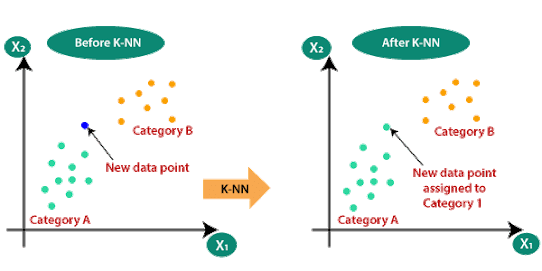
\includegraphics[scale=.6]{IMG_8202.png}}
\caption{KNN}
\end{figure}
\end{center}

The Euclidian Distance function goes as : 
\begin{equation*}
D=\sqrt{\sum_{i=1}^{k}{(x_i - y_i)^2}}
\end{equation*}

This gives the model the mean euclidian distance in a set of '$k$' points 

It should also be noted that all three distance measures are only valid for continuous variables. In the instance of categorical variables the Hamming distance must be used. It also brings up the issue of standardization of the numerical variables between 0 and 1 when there is a mixture of numerical and categorical variables in the dataset.

Choosing the optimal value for K is best done by first inspecting the data. In general, a large K value is more precise as it reduces the overall noise but there is no guarantee. Cross-validation is another way to retrospectively determine a good K value by using an independent dataset to validate the K value. Historically, the optimal K for most datasets has been between 3-10.

\begin{center}
\begin{figure}[h]
\centerline{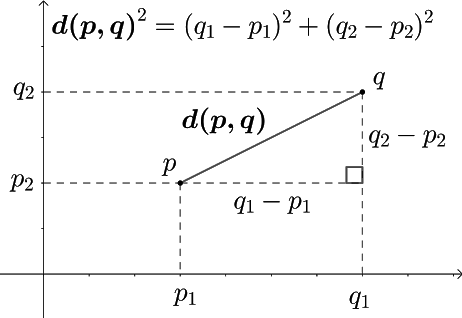
\includegraphics[scale=.5]{IMG_8203.png}}
\caption{Euclidian Distance}
\end{figure}
\end{center}

KNN is a type of instance-based learning, or lazy learning, where the function is only approximated locally and all computation is deferred until function evaluation. Since this algorithm relies on distance for classification, normalizing the training data can improve its accuracy dramatically.

Both for classification and regression, a useful technique can be to assign weights to the contributions of the neighbors, so that the nearer neighbors contribute more to the average than the more distant ones. For example, a common weighting scheme consists in giving each neighbor a weight of :  
\begin{equation*}
\frac{1}{d}
\end{equation*}
where $d$ is the distance to the neighbor.
The neighbors are taken from a set of objects for which the class or the object property value is known. This can be thought of as the training set for the algorithm, though no explicit training step is required.

A peculiarity of the KNN algorithm is that it is sensitive to the local structure of the data.
\newpage
\subsection{\msize{\textbf{LOGISTIC REGRESSION}}}
Logistic regression is a statistical model that in its basic form uses a logistic function to model a binary dependent variable, although many more complex extensions exist. In regression analysis, logistic regression s estimating the parameters of a logistic model. Mathematically, a binary logistic model has a dependent variable with two possible values, such as pass/fail which is represented by an indicator variable, where the two values are labeled "0" and "1". In the logistic model, the log-odds  for the value labeled "1" is a linear combination of one or more independent variables the independent variables can each be a binary variable (two classes, coded by an indicator variable) or a continuous variable. The corresponding probability of the value labeled "1" can vary between 0 and 1, hence the labeling; the function that converts log-odds to probability is the logistic function, hence the name.

In a binary logistic regression model, the dependent variable has two levels. Outputs with more than two values are modeled by multinomial logistic regression and, if the multiple categories are ordered, by ordinal logistic regression. The logistic regression model itself simply models probability of output in terms of input and does not perform statistical classification though it can be used to make a classifier, for instance by choosing a cutoff value and classifying inputs with probability greater than the cutoff as one class, below the cutoff as the other; this is a common way to make a binary classifier. The coefficients are generally not computed by a closed-form expression, unlike linear least squares

The activation function of a logistic regression is a simple sigmoid. The sigmoid is given by : 
\begin{equation*} 
sigmoid= \frac{1}{1+e^{-x}}
\end{equation*}
For all '$x$' in our given dataset 

\begin{center}
\begin{figure}[h]
\centerline{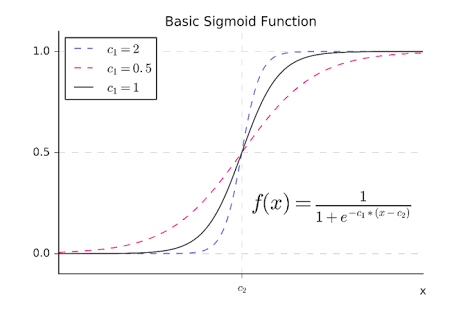
\includegraphics[scale=.7]{IMG_8204.png}}
\caption{Sigmoid Function}
\end{figure}
\end{center}

using the sigmoid activation function and its derivatives, the model fits the given data to a logistic curve which is the result of our classification technique. 

Logistic regression models the probability of the default class.For example, if we are modeling people’s sex as male or female from their height, then the first class could be male and the logistic regression model could be written as the probability of male given a person’s height

Some of the limitations of logistic regression are : 

1. Binary Output Variable: This might be obvious as we have already mentioned it, but logistic regression is intended for binary (two-class) classification problems. It will predict the probability of an instance belonging to the default class, which can be snapped into a 0 or 1 classification.

2. Remove Noise: Logistic regression assumes no error in the output variable, consider removing outliers and possibly misclassified instances from your training data.

3.Gaussian Distribution: Logistic regression is a linear algorithm (with a non-linear transform on output). It does assume a linear relationship between the input variables with the output. Data transforms of your input variables that better expose this linear relationship can result in a more accurate model. For example, you can use log, root, Box-Cox and other univariate transforms to better expose this relationship.

4. Remove Correlated Inputs: Like linear regression, the model can overfit if you have multiple highly-correlated inputs. Consider calculating the pairwise correlations between all inputs and removing highly correlated inputs. 

5. Fail to Converge: It is possible for the expected likelihood estimation process that learns the coefficients to fail to converge. This can happen if there are many highly correlated inputs in your data or the data is very sparse 
\newpage
\subsection{\msize{\textbf{DECISION TREES}}}
A decision tree is a flowchart-like structure in which each internal node represents a test on an attribute, each branch represents the outcome of the test, and each leaf node represents a class label. The paths from root to leaf represent classification rules.

In decision analysis, a decision tree and the closely related influence diagram are used as a visual and analytical decision support tool, where the expected values (or expected utility) of competing alternatives are calculated.

A decision tree consists of three types of nodes : 

1. Decision nodes – typically represented by squares

2. Chance nodes – typically represented by circles

3. End nodes – typically represented by triangles

The decision tree can be linearized into decision rules where the outcome is the contents of the leaf node, and the conditions along the path form a conjunction in the if clause. In general, the rules have the form

As a problem usually has a large set of features, it results in large number of split, which in turn gives a huge tree. Such trees are complex and can lead to overfitting. So, we need to know when to stop? One way of doing this is to set a minimum number of training inputs to use on each leaf. For example we can use a minimum of 10 passengers to reach a decision(died or survived), and ignore any leaf that takes less than 10 passengers. Another way is to set maximum depth of your model. Maximum depth refers to the the length of the longest path from a root to a leaf.

\begin{center}
\begin{figure}[h]
\centerline{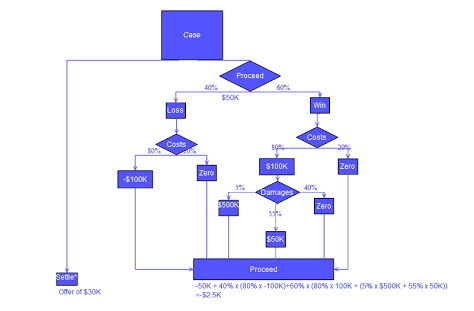
\includegraphics[scale=.7]{IMG_8205.jpg}}
\caption{Decision Trees}
\end{figure}
\end{center}

The performance of a tree can be further increased by pruning. It involves removing the branches that make use of features having low importance. This way, we reduce the complexity of tree, and thus increasing its predictive power by reducing overfitting.

Pruning can start at either root or the leaves. The simplest method of pruning starts at leaves and removes each node with most popular class in that leaf, this change is kept if it doesn't deteriorate accuracy. Its also called reduced error pruning. More sophisticated pruning methods can be used such as cost complexity pruning where a learning parameter (alpha) is used to weigh whether nodes can be removed based on the size of the sub-tree. This is also known as weakest link pruning.

The advantages include: 

1. Simple to understand, interpret, visualize

2. Decision trees implicitly perform variable screening or feature selection

3. Can handle both numerical and categorical data. Can also handle multi-output problems.

4. Nonlinear relationships between parameters do not affect tree performance

The disadvantages include : 

1. Decision-tree learners can create over-complex trees that do not generalize the data well. This is called overfitting.

2. Decision trees can be unstable because small variations in the data might result in a completely different tree being generated. This is called variance, which needs to be lowered by methods like bagging and boosting

3. Greedy algorithms cannot guarantee to return the globally optimal decision tree. This can be mitigated by training multiple trees, where the features and samples are randomly sampled with replacement.

4. Decision tree learners create biased trees if some classes dominate. It is therefore recommended to balance the data set prior to fitting with the decision tree
\newpage 

\subsection{\msize{\textbf{RANDOM FOREST CLASSIFIER}}}
Random forests or random decision forests are an ensemble learning method for classification, regression and other tasks that operate by constructing a multitude of decision trees at training time and outputting the class that is the mode of the classes (classification) or mean/average prediction (regression) of the individual trees

Random decision forests correct for decision trees' habit of overfitting to their training set. Random forests generally outperform decision trees, but their accuracy is lower than gradient boosted trees. However, data characteristics can affect their performance.

In particular, trees that are grown very deep tend to learn highly irregular patterns: they overfit their training sets, i.e. have low bias, but very high variance. Random forests are a way of averaging multiple deep decision trees, trained on different parts of the same training set, with the goal of reducing the variance.[3]:587–588 This comes at the expense of a small increase in the bias and some loss of interpretability, but generally greatly boosts the performance in the final model.

Forests are like the pulling together of decision tree algorithm efforts. Taking the teamwork of many trees thus improving the performance of a single random tree. Though not quite similar, forests give the effects of a K-fold cross validation.

The bagging formula is given by : 

\begin{equation*} 
f^{~}= \frac{1}{B}\sum_{b=1}^{B}{f_b(x^{'})}
\end{equation*}

This bootstrapping procedure leads to better model performance because it decreases the variance of the model, without increasing the bias. This means that while the predictions of a single tree are highly sensitive to noise in its training set, the average of many trees is not, as long as the trees are not correlated. Simply training many trees on a single training set would give strongly correlated trees (or even the same tree many times, if the training algorithm is deterministic); bootstrap sampling is a way of de-correlating the trees by showing them different training sets.

\begin{center}
\begin{figure}[h]
\centerline{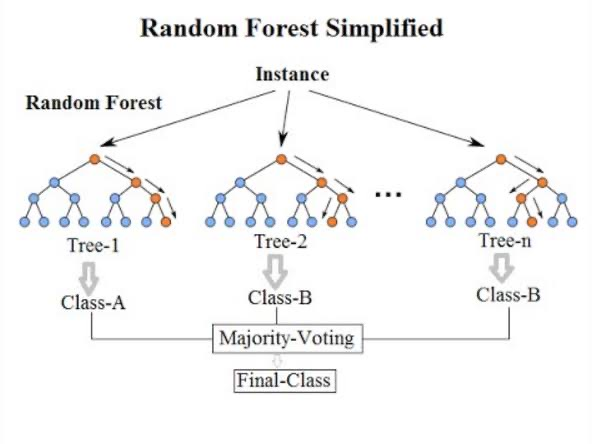
\includegraphics[scale=.5]{IMG_8206.jpg}}
\caption{Random Forests}
\end{figure}
\end{center}

Additionally, an estimate of the uncertainty of the prediction can be made as the standard deviation of the predictions from all the individual regression trees on $x$ 

\begin{equation*}
\sigma= \sqrt{\frac{\sum_{b=1}^{B}{(f_b(x^{'})-f)^{2}}}{B-1}}
\end{equation*}

The number of samples/trees, B, is a free parameter. Typically, a few hundred to several thousand trees are used, depending on the size and nature of the training set. An optimal number of trees B can be found using cross-validation, or by observing the out-of-bag error: t

The advantages of this are : 

1. It reduces overfitting in decision trees and helps to improve the accuracy

2. It is flexible to both classification and regression problems

3. It works well with both categorical and continuous values

4. Normalising of data is not required as it uses a rule-based approach.

The disadvantages include : 

1. It requires much computational power as well as resources as it builds numerous trees to combine their outputs. 

2. It also requires much time for training as it combines a lot of decision trees to determine the class.

3. Due to the ensemble of decision trees, it also suffers interpretability and fails to determine the significance of each variable.
\newpage 
\subsection{\msize{\textbf{SUPPORT VECTOR MACHINES}}}
Support vector machine is highly preferred by many as it produces significant accuracy with less computation power. Support Vector Machine, abbreviated as SVM can be used for both regression and classification tasks. But, it is widely used in classification objectives.

The objective of the support vector machine algorithm is to find a hyperplane in an N-dimensional space(N — the number of features) that distinctly classifies the data points. To separate the two classes of data points, there are many possible hyperplanes that could be chosen. Our objective is to find a plane that has the maximum margin, i.e the maximum distance between data points of both classes. Maximizing the margin distance provides some reinforcement so that future data points can be classified with more confidence.

Hyperplanes are decision boundaries that help classify the data points. Data points falling on either side of the hyperplane can be attributed to different classes. Also, the dimension of the hyperplane depends upon the number of features. If the number of input features is 2, then the hyperplane is just a line. If the number of input features is 3, then the hyperplane becomes a two-dimensional plane. It becomes difficult to imagine when the number of features exceeds 3.

\begin{center}
\begin{figure}[h]
\centerline{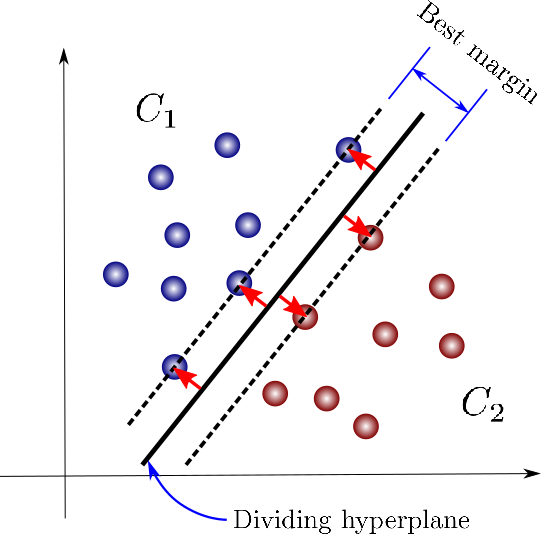
\includegraphics[scale=.35]{IMG_8207.png}}
\caption{Support Vector Machines}
\end{figure}
\end{center}

In logistic regression, we take the output of the linear function and squash the value within the range of [0,1] using the sigmoid function. If the squashed value is greater than a threshold value(0.5) we assign it a label 1, else we assign it a label 0. In SVM, we take the output of the linear function and if that output is greater than 1, we identify it with one class and if the output is -1, we identify is with another class. Since the threshold values are changed to 1 and -1 in SVM, we obtain this reinforcement range of values([-1,1]) which acts as margin.

In the SVM algorithm, we are looking to maximize the margin between the data points and the hyperplane. The loss function that helps maximize the margin is hinge loss : 

\begin{equation*}
c(x,y,f(x))=(1-y*f(x))_{+}
\end{equation*}

This is the hinge loss function. The cost is 0 if the predicted value and the actual value are of the same sign. If they are not, we then calculate the loss value. We also add a regularization parameter the cost function. The objective of the regularization parameter is to balance the margin maximization and loss. After adding the regularization parameter, the cost functions looks as below :

\begin{equation*} 
min_{w} \lambda ||w||^{2} + \sum_{i=1}^{n}{(1-y_i <x_i,w>)_+}
\end{equation*}

When there is a misclassification, i.e our model make a mistake on the prediction of the class of our data point, we include the loss along with the regularization parameter to perform gradient update.

The advantages include : 

1. SVM works relatively well when there is a clear margin of separation between classes.

2. SVM is more effective in high dimensional spaces.

3. SVM is effective in cases where the number of dimensions is greater than the number of samples.


4. SVM is relatively memory efficient

The disadvantages include : 

1. SVM algorithm is not suitable for large data sets.

2. SVM does not perform very well when the data set has more noise i.e. target classes are overlapping.

3. In cases where the number of features for each data point exceeds the number of training data samples, the SVM will underperform.

4. As the support vector classifier works by putting data points, above and below the classifying hyperplane there is no probabilistic explanation for the classification.
\newpage
\section{\mainsize{\textbf{IMPLEMENTATION}}}
We have implemented and deployed all the said machine learning algorithms in the Juputer Notebook environment based on Python 3.8.3 version. 

We have also used the SciKit- Learn library for implementing the model as well as pandas for the dataset manipulation and Matplotlib for visual analysis 
\subsection{\msize{\textbf{THE DATA-SET}}}
We have procurred the data set from an online open source github $\text{repository}^{[6]}$. We tried to acess the local hospitals with the hope that they could provide us the live data-set but unfortunately due to the recent pandemic crisis, their plate was full and were not able to help us 

The data-set we used is a huge dataset which contains 568 rows and 32 columns which amounts to 18,176 cells of data. 

This data is decompressed form of various computer tomography scans and contains information such as : radius mean	texture mean, perimeter mean, area mean, smoothness mean, compactness mean, concavity mean and so on 


This data is clear of any noise and is ready to be passed through our model 
\newpage
\subsection{\msize{\textbf{PYTHON}}}
Python is an interpreted, high-level and general-purpose programming language. Python's design philosophy emphasizes code readability with its notable use of significant whitespace.

Python is dynamically typed and garbage-collected. It supports multiple programming paradigms, including structured (particularly, procedural), object-oriented, and functional programming. Python is often described as a "batteries included" language due to its comprehensive standard library.

\begin{center}
\begin{figure}[h]
\centerline{
\includegraphics[scale=.7]{IMG_8208.png}}
\caption{Python Logo}
\end{figure}
\end{center}

Python interpreters are supported for mainstream operating systems and available for a few more (and in the past supported many more). A global community of programmers develops and maintains CPython, a free and open-source[31] reference implementation. A non-profit organization, the Python Software Foundation, manages and directs resources for Python and CPython development. It currently ties with Java as the second most popular programming language in the world.
\newpage
\subsection{\msize{\textbf{JUPYTER NOTEBOOK}}}
JupyterLab is a web-based interactive development environment for Jupyter notebooks, code, and data. JupyterLab is flexible: configure and arrange the user interface to support a wide range of workflows in data science, scientific computing, and machine learning. JupyterLab is extensible and modular: write plugins that add new components and integrate with existing ones.

\begin{center}
\begin{figure}[h]
\centerline{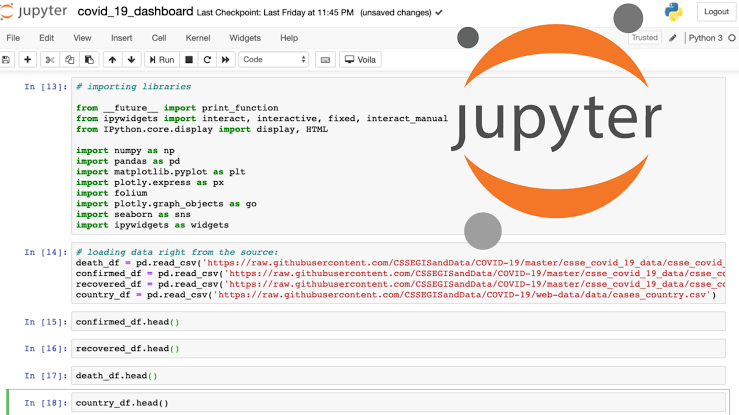
\includegraphics[scale=.5]{IMG_8209.png}}
\caption{Jupyter Notebook}
\end{figure}
\end{center}

Jupyter supports over 40 programming languages, including Python, R, Julia, and Scala. Notebooks can be shared with others using email, Dropbox, GitHub and the Jupyter Notebook Viewer. Your code can produce rich, interactive output: HTML, images, videos, LaTeX, and custom MIME types. Leverage big data tools, such as Apache Spark, from Python, R and Scala. Explore that same data with pandas, scikit-learn, ggplot2, TensorFlow.
\newpage
\subsection{\msize{\textbf{SCIKIT LEARN }}}
Scikit-learn (formerly scikits.learn and also known as sklearn) is a free software machine learning library for the Python programming language.[2] It features various classification, regression and clustering algorithms including support vector machines, random forests, gradient boosting, k-means and DBSCAN, and is designed to interoperate with the Python numerical and scientific libraries NumPy and SciPy.

\begin{center}
\begin{figure}[h]
\centerline{
\includegraphics[scale=.15]{IMG_8210.png}}
\caption{Scikit Learn}
\end{figure}
\end{center}

 
Scikit-learn is largely written in Python, and uses numpy extensively for high-performance linear algebra and array operations. Furthermore, some core algorithms are written in Cython to improve performance. Support vector machines are implemented by a Cython wrapper around LIBSVM; logistic regression and linear support vector machines by a similar wrapper around LIBLINEAR. In such cases, extending these methods with Python may not be possible.

Scikit-learn integrates well with many other Python libraries, such as matplotlib and plotly for plotting, numpy for array vectorization, pandas dataframes, scipy, and many more.
\newpage
\subsection{\msize{\textbf{PANDAS}}}
In computer programming, pandas is a software library written for the Python programming language for data manipulation and analysis. In particular, it offers data structures and operations for manipulating numerical tables and time series. It is free software released under the three-clause BSD license.

The name is derived from the term "panel data", an econometrics term for data sets that include observations over multiple time periods for the same individuals.

\begin{center}
\begin{figure}[h]
\centerline{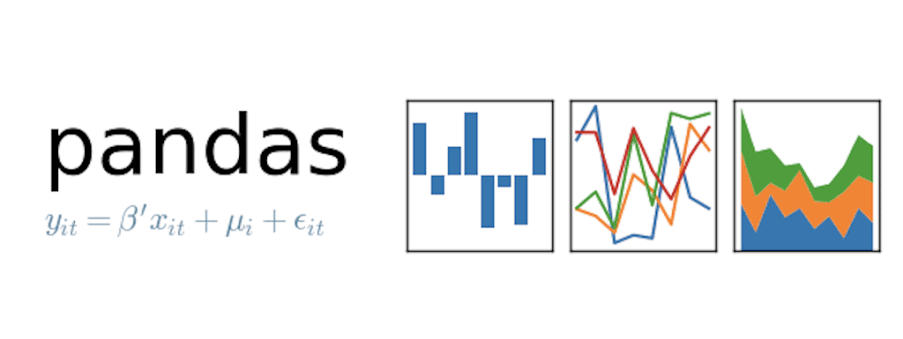
\includegraphics[scale=.4]{IMG_8211.png}}
\caption{Pandas}
\end{figure}
\end{center}

Pandas is mainly used for data analysis. Pandas allows importing data from various file formats such as comma-separated values, JSON, SQL, Microsoft Excel. Pandas allows various data manipulation operations such as merging, reshaping, selecting, as well as data cleaning, and data wrangling features.
\newpage
\subsection{\msize{\textbf{MATPLOTLIB}}}
Matplotlib is a plotting library for the Python programming language and its numerical mathematics extension NumPy. It provides an object-oriented API for embedding plots into applications using general-purpose GUI toolkits like Tkinter, wxPython, Qt, or GTK+. There is also a procedural "pylab" interface based on a state machine (like OpenGL), designed to closely resemble that of MATLAB, though its use is discouraged.

Pyplot is a Matplotlib module which provides a MATLAB-like interface. Matplotlib is designed to be as usable as MATLAB, with the ability to use Python, and the advantage of being free and open-source.

\begin{center}
\begin{figure}[h]
\centerline{
\includegraphics[scale=.7]{IMG_8212.png}}
\caption{Matplotlib}
\end{figure}
\end{center}

Overall toolkits are available which extend Matplotlib functionality. Some are separate downloads, others ship with the Matplotlib source code but have external dependencies. 

\newpage
\section{\mainsize{\textbf{TESTING AND VALIDATION}}}
We have implemented and deployed all the five machine learning models in the jupyter development environment and have tested these models rigorously over a varying level of epochs. We have split the original data set into training and testing data. 

The data set is first split into X and Y labels. The X label holds all the various inputs that we want to pass to the model. The Y label includes the target output which is whether the tumour in malignant or benign 

These X and Y labels are again split into X-Train And X-Test, Y-Train and Y-Test parts. The X-train and Y-train are initially used to train the model and the X-test and Y-test is used to test the model 
\,
\,
\,
\begin{center}
\begin{figure}[h]
\centerline{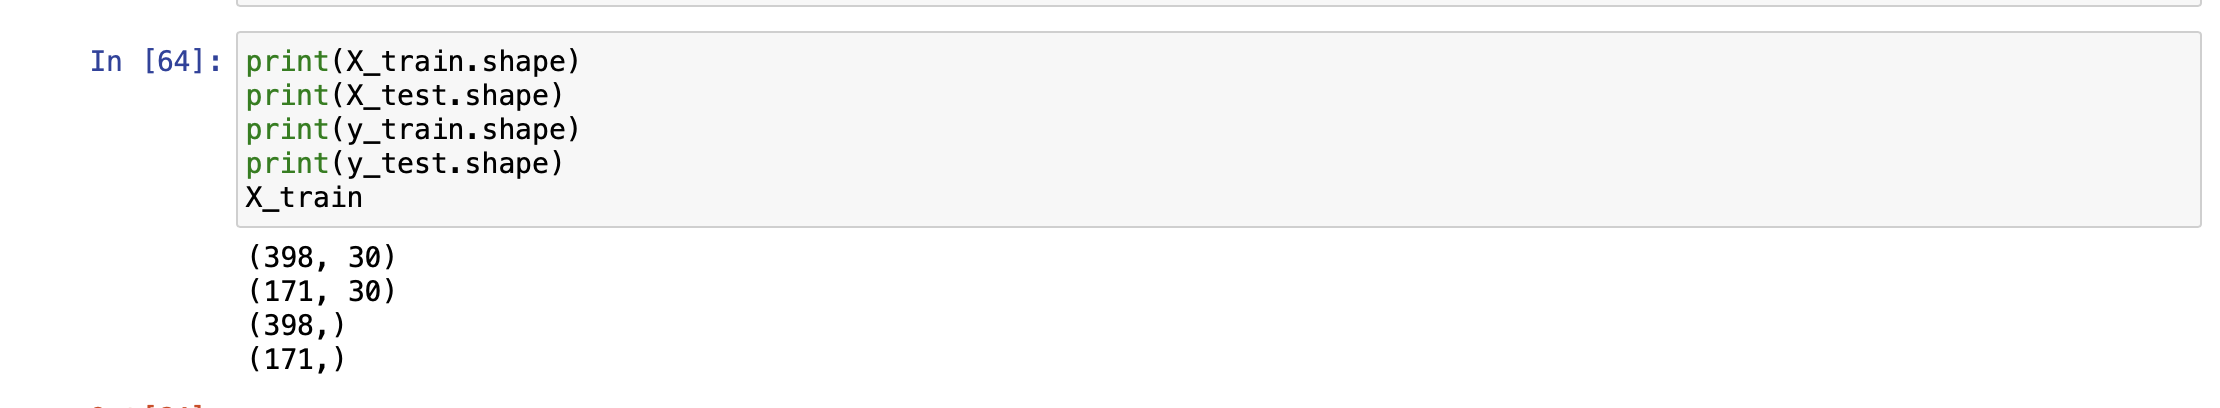
\includegraphics[scale=.5]{aft-split.png}}
\caption{Training and Testing set}
\end{figure}
\end{center}

The above code snippet shows the number of rows and columns in each of the training and testing attribute dataset 
\newpage 
\subsection{\msize{\textbf{TRAINING AND TESTING SPLIT}}}
The original dataset is split with a 7:3 ratio among the training and testing datasets. This means that 70\% of the dataset constitute the X-train and Y-train attributes and 30\% of the dataset contributes to the X-test and Y-test attributes 

Splitting the dataset with a 7:3 ratio ensures that we have a large amount of data to test the models accurately. The data set is first split into X and Y labels. The X label holds all the various inputs that we want to pass to the model. The Y label includes the target output which is whether the tumour in malignant or benign 

\begin{center}
\begin{figure}[h]
\centerline{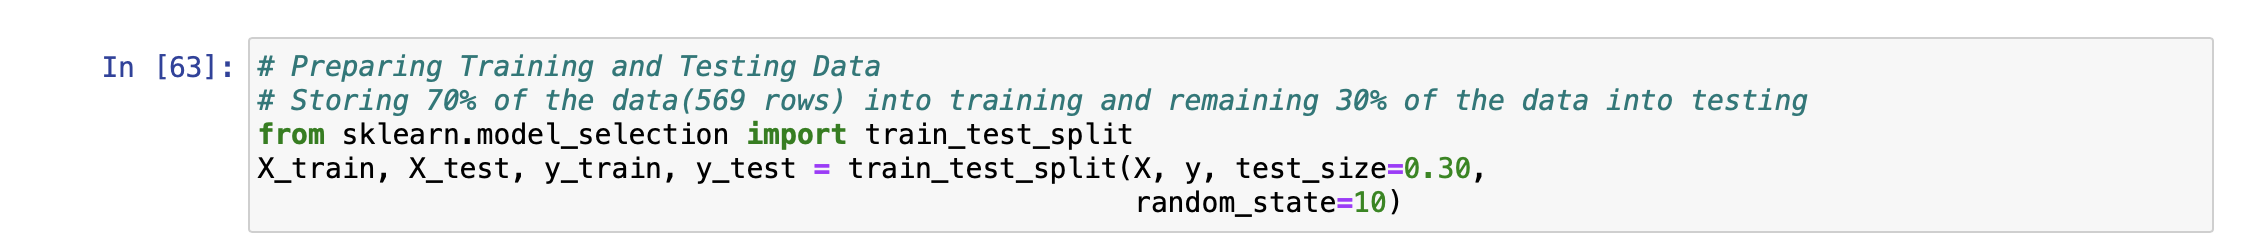
\includegraphics[scale=.5]{splitt.png}}
\caption{Split ratio}
\end{figure}
\end{center}

These X and Y labels are again split into X-Train And X-Test, Y-Train and Y-Test parts. The X-train and Y-train are initially used to train the model and the X-test and Y-test is used to test the model 
\newpage 
\subsection{\msize{\textbf{VISUAL ANALYSIS}}}
We have used the matplotlib and pandas library to get a visual intuition of the dataset. We have formed a co-relation graph which gives us a heat map of how each attribute in our dataset is linked to each other. This gives us a measure of how much of which attributes affect out output classification the most which can help in future debugging 	 

\begin{center}
\begin{figure}[h]
\centerline{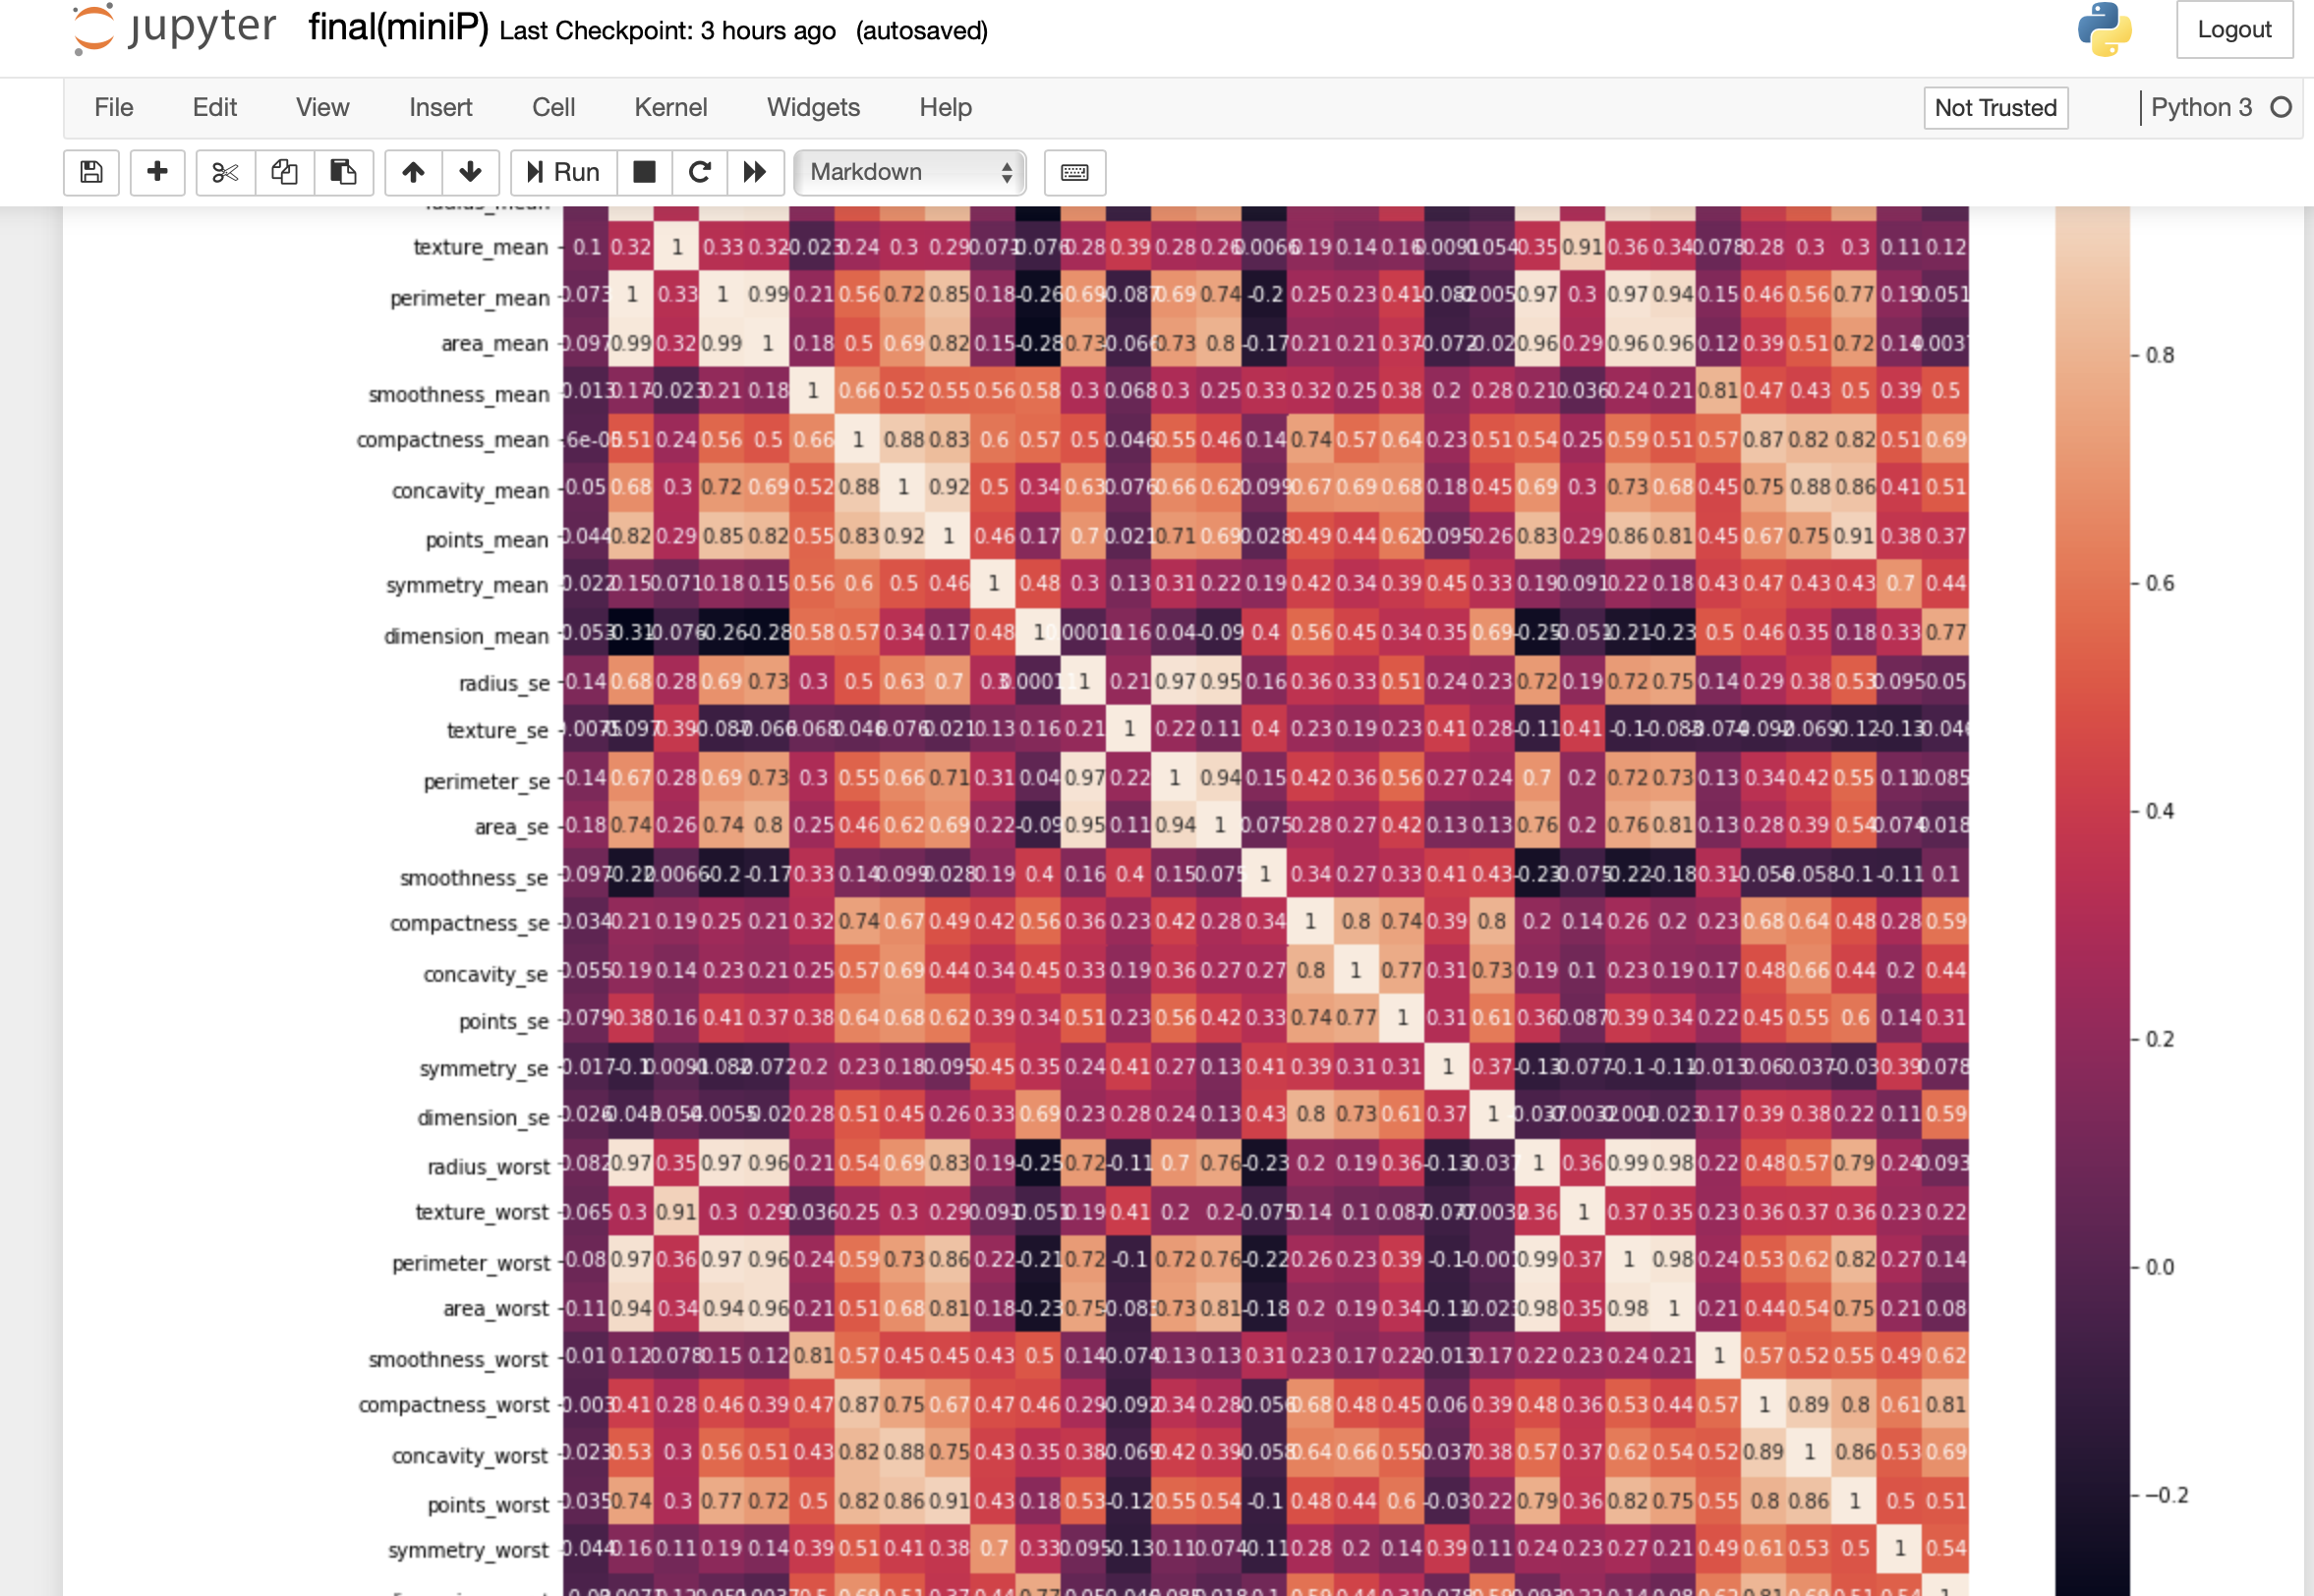
\includegraphics[scale=.4]{co.png}}
\caption{Co-relation matrix}
\end{figure}
\end{center}

As we observe the heat map of co-relations, the values will range from between -1 to +1. A value of 0 indicates no co-relation, a value of -1 indicates negative co-relation and a value of +1 indicates that the data is highly co-related 

\begin{center}
\begin{figure}[h]
\centerline{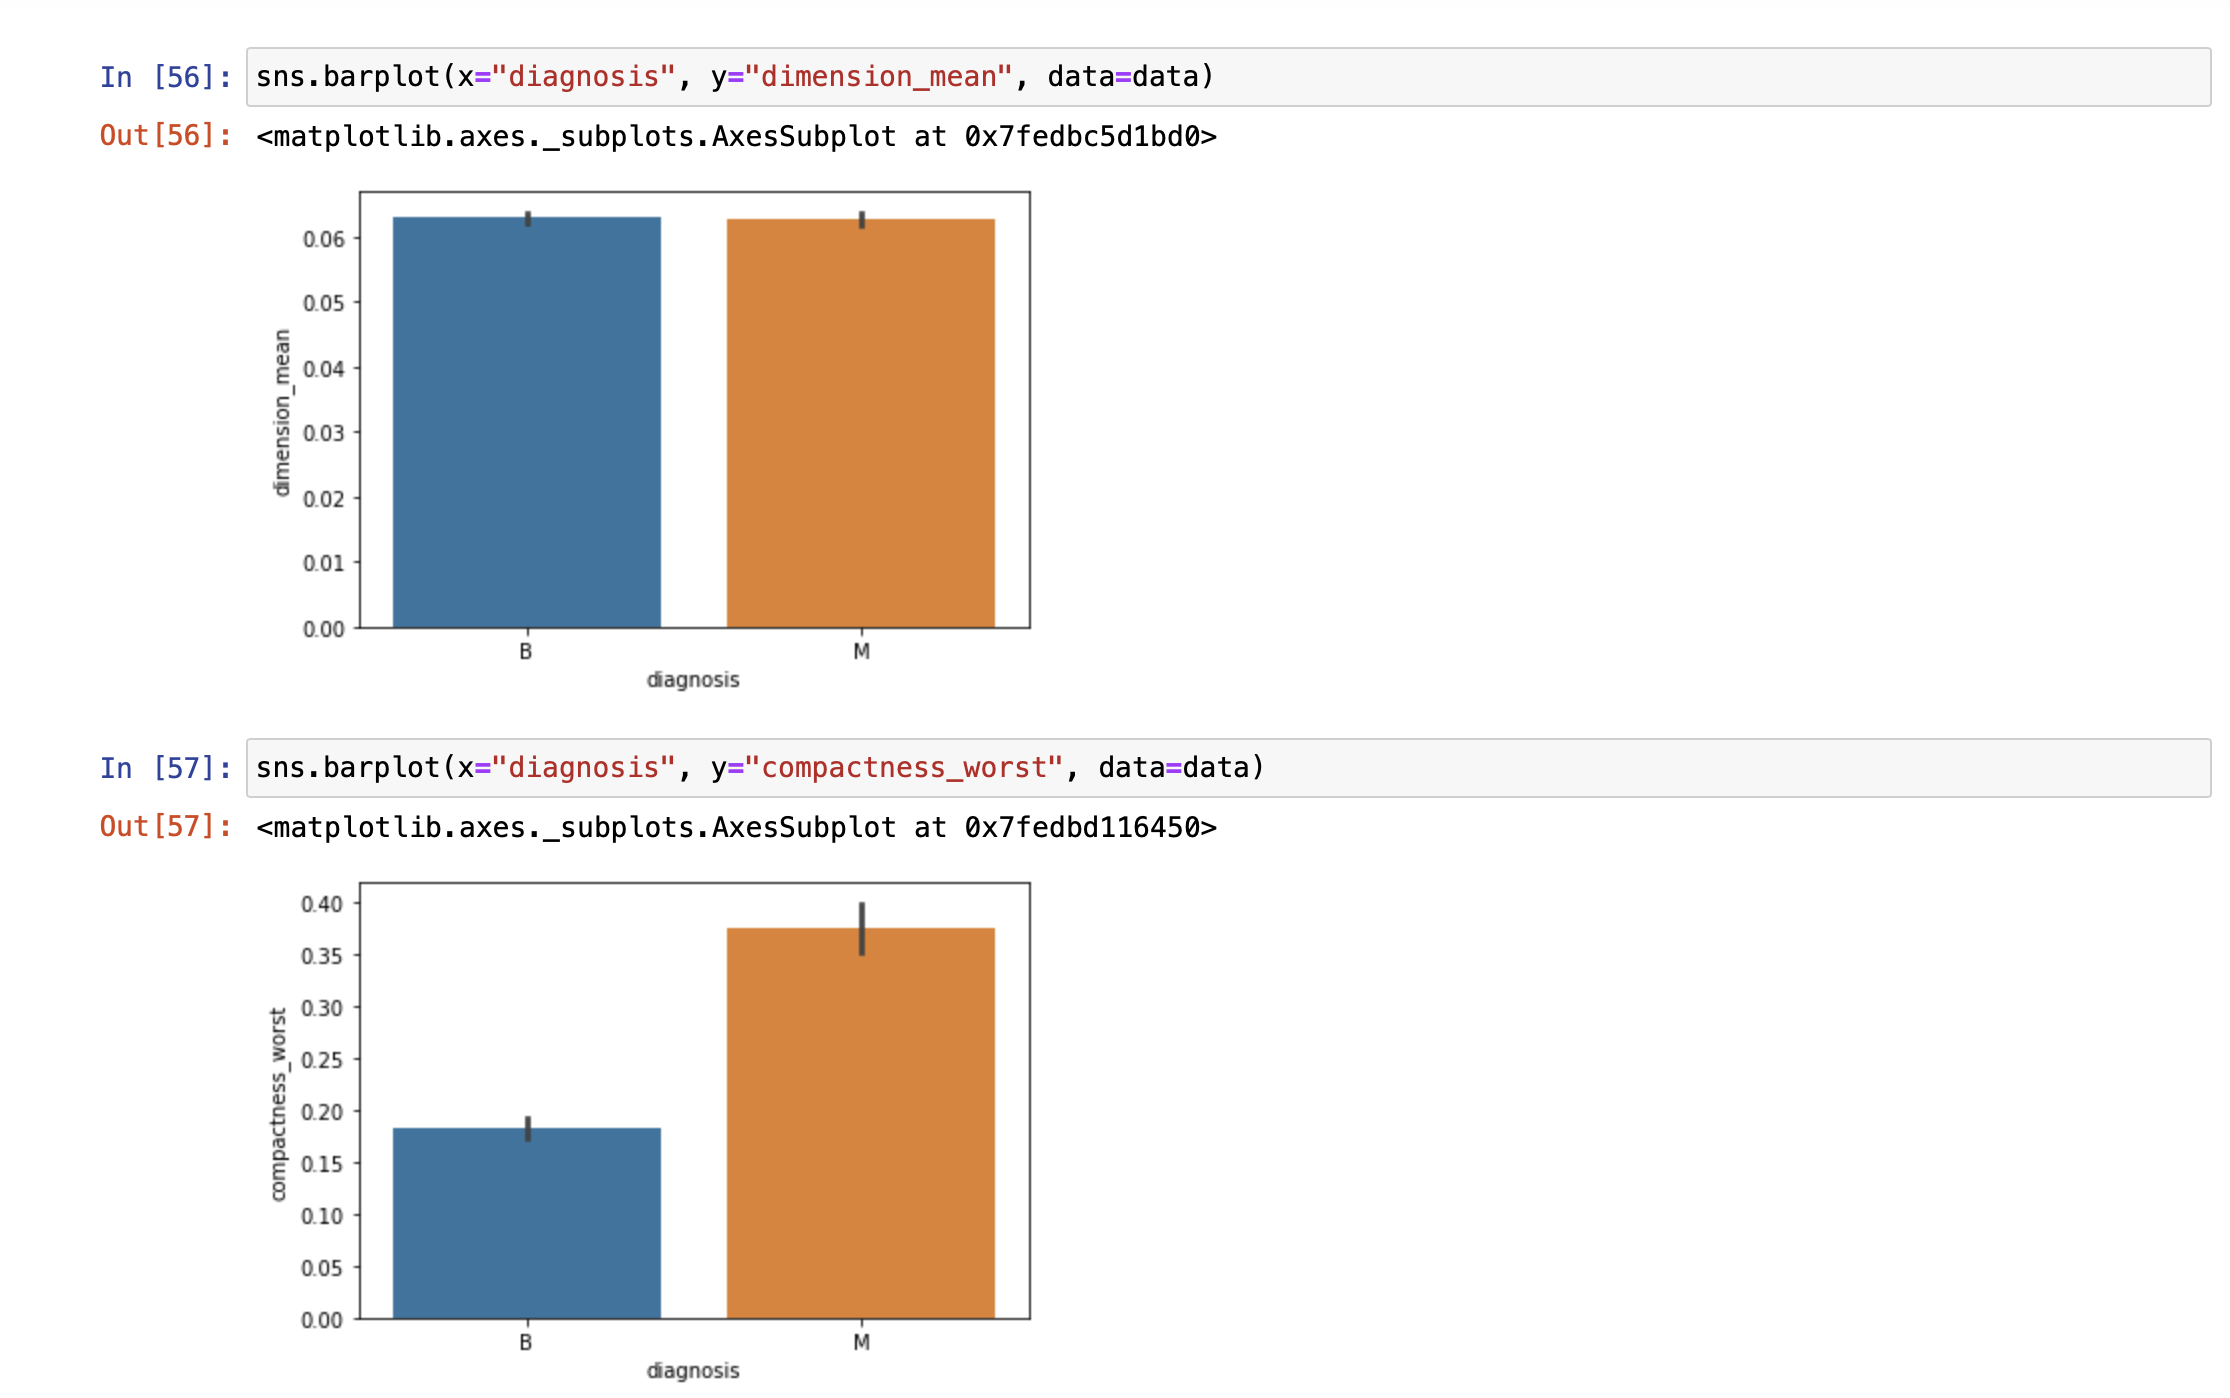
\includegraphics[scale=.4]{co2.png}}
\caption{Bar Plots}
\end{figure}
\end{center}

We have also plotted some bar graphs which help us understand certain attributes contribution to the output in a much better way 

\newpage
\subsection{\msize{\textbf{TESTING THE MODELS}}}
Here we will. be training and testing all the five machine learning algorithms:
\subsubsection{\textbf{K NEAREST NEIGHBOURS }}
The KNN has been implemented using the KNeighborsClassifier from the sklearn.neighbors library. We have also used the Euclidian distance function as cited in the previous sections 

\begin{center}
\centerline{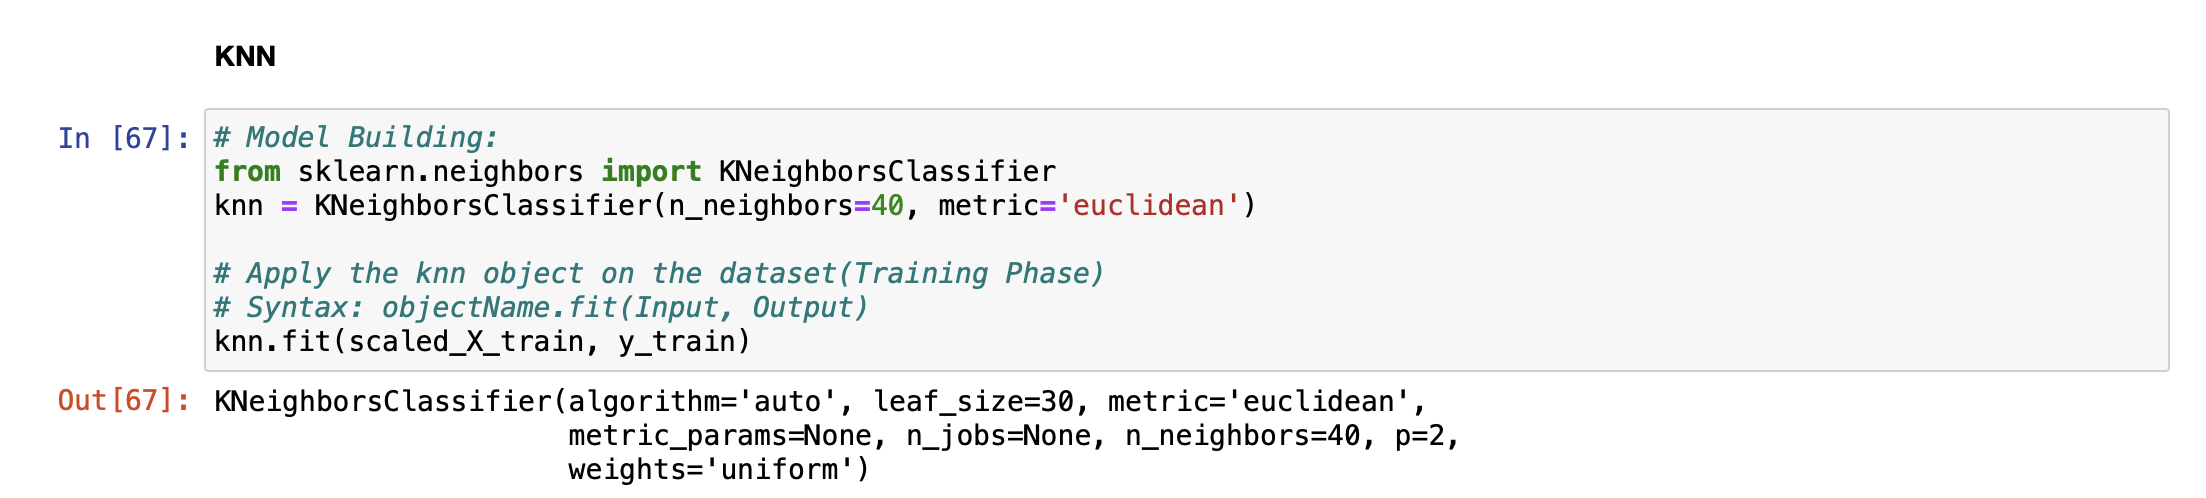
\includegraphics[scale=.4]{knn.png}}
\end{center}

The testing is done in the following manner

\begin{center}
\begin{figure}[h]
\centerline{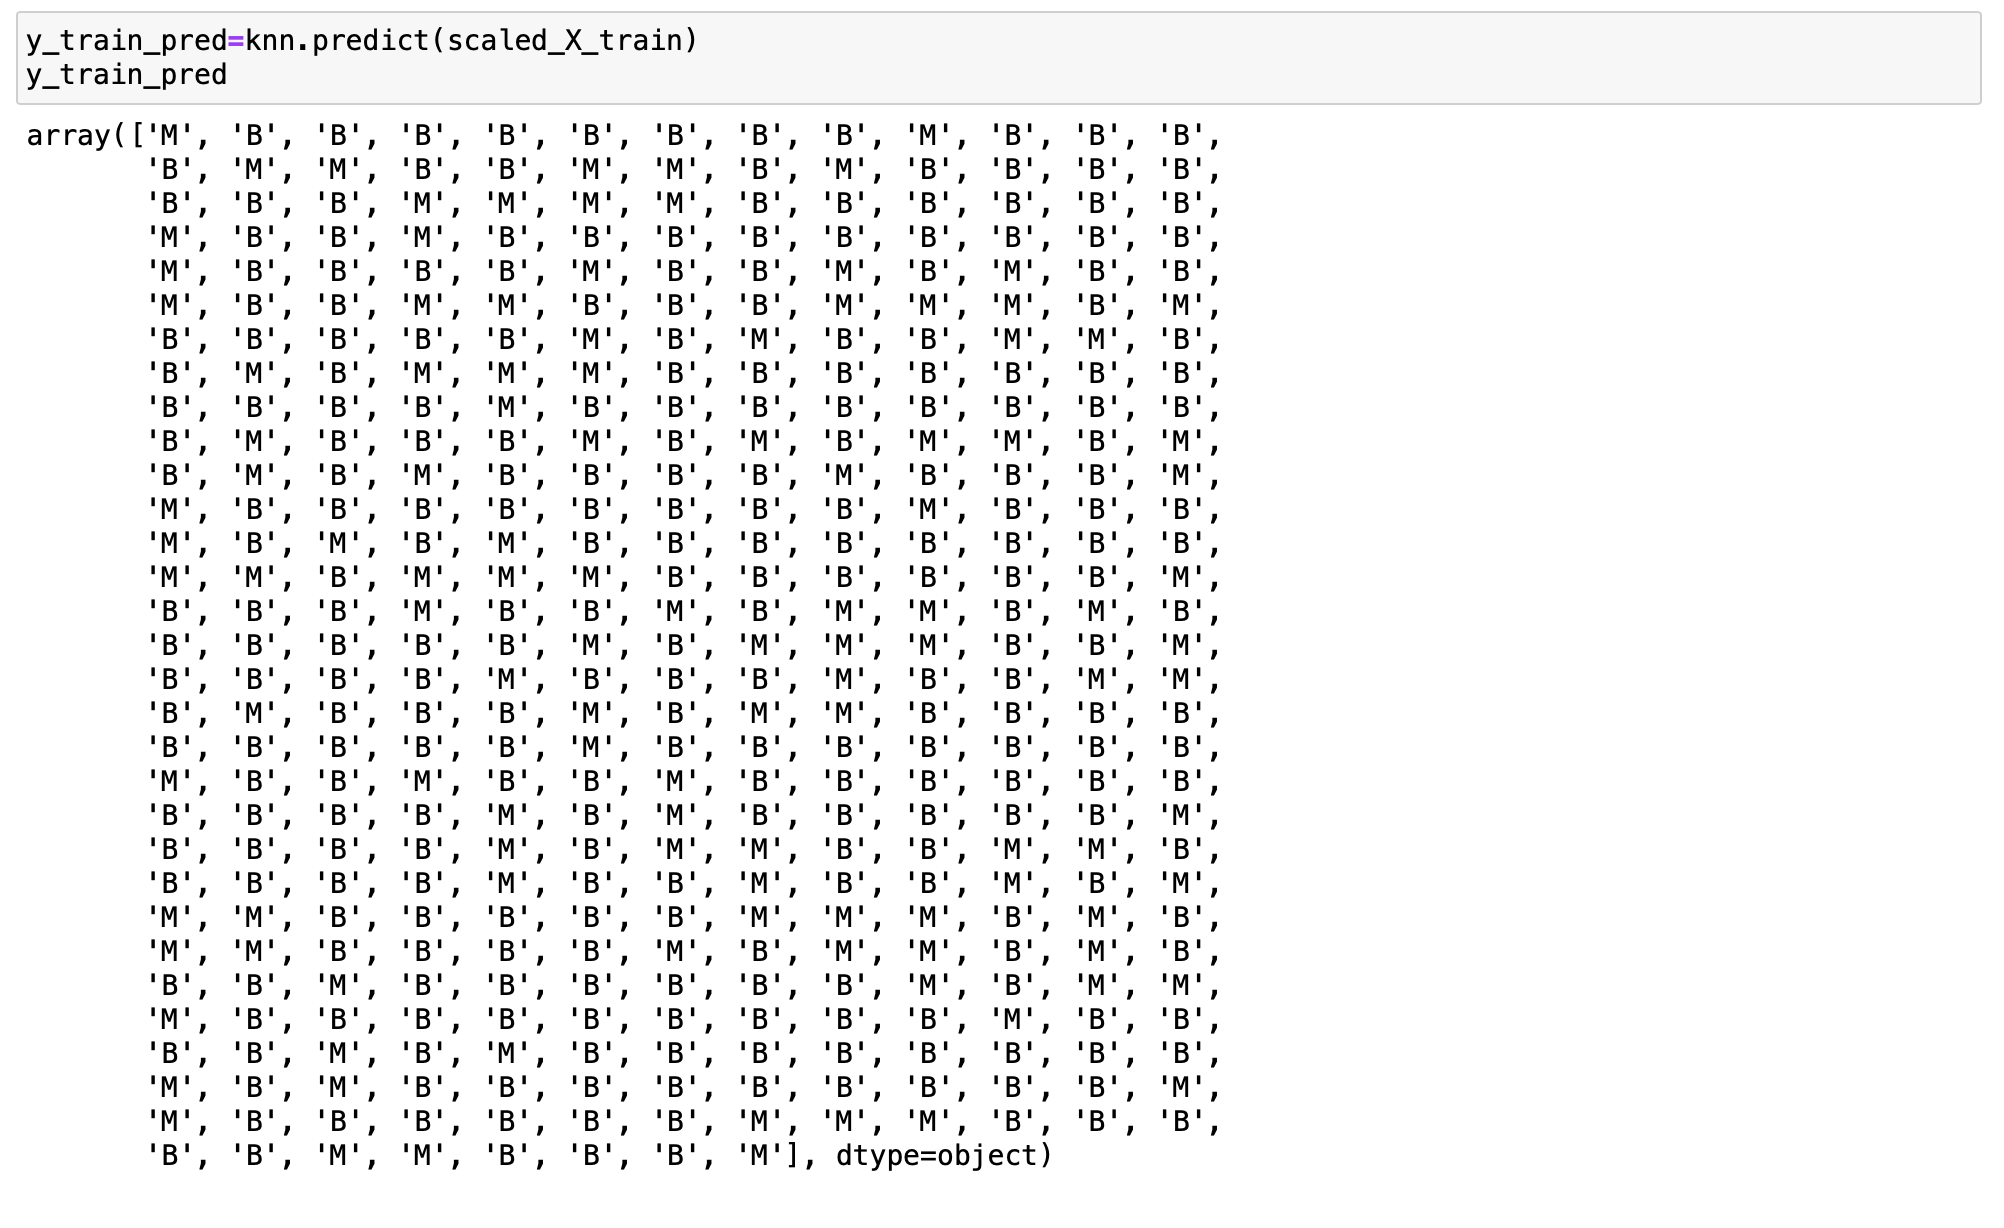
\includegraphics[scale=.4]{knnpred.png}}
\caption{Knn Prediction}
\end{figure}
\end{center}

\newpage
\subsubsection{\textbf{LOGISTIC REGRESSION }}
The logistic regression is implemented using the LogisticRegression class of the sklearn.linear-model model. In this we will be fitting our training and testing data

\begin{center}
\centerline{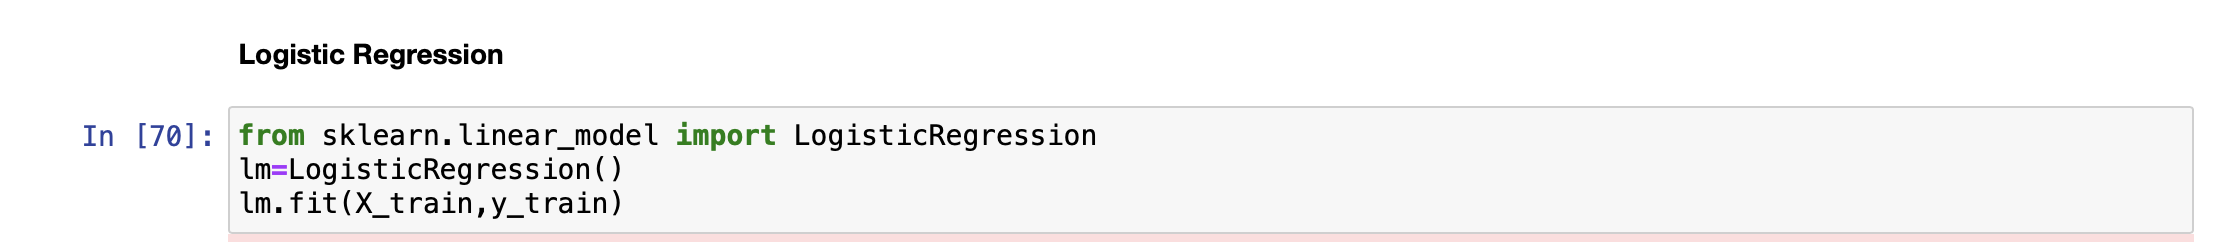
\includegraphics[scale=.4]{lr.png}}
\end{center}

\begin{center}
\centerline{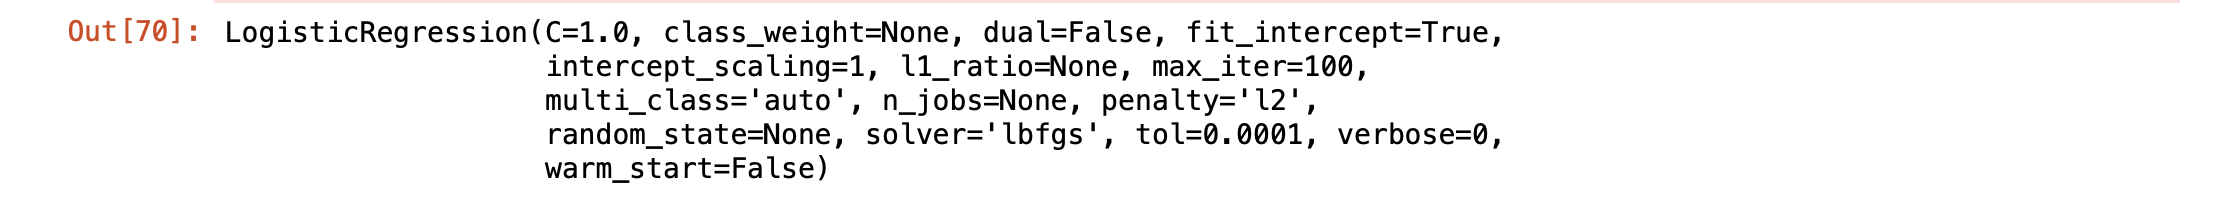
\includegraphics[scale=.4]{lr2.png}}
\end{center}

The testing for logisitic regresion is done as: 

\begin{center}
\begin{figure}[h]
\centerline{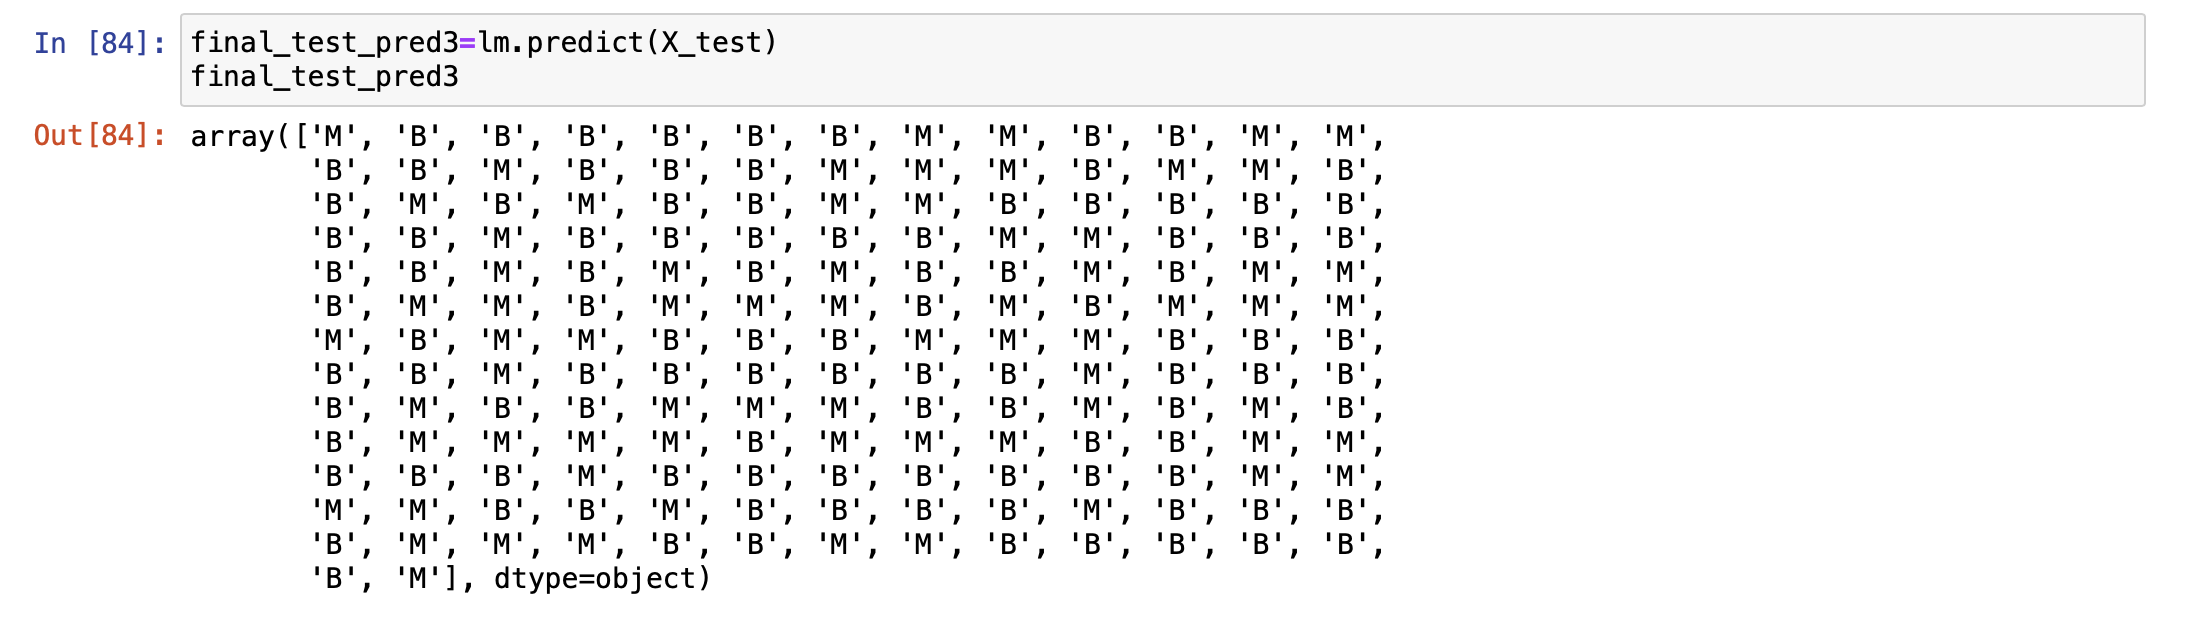
\includegraphics[scale=.4]{lrtest.png}}
\caption{Logistic Regression Prediction}
\end{figure}
\end{center}
\newpage 

\subsubsection{\textbf{DECISION TREE }}
The Decision Tree is implemented using the DecisionTreeClassifier class from the sklearn-tree model. The training and testing data is fit to it as follows 

\begin{center}
\centerline{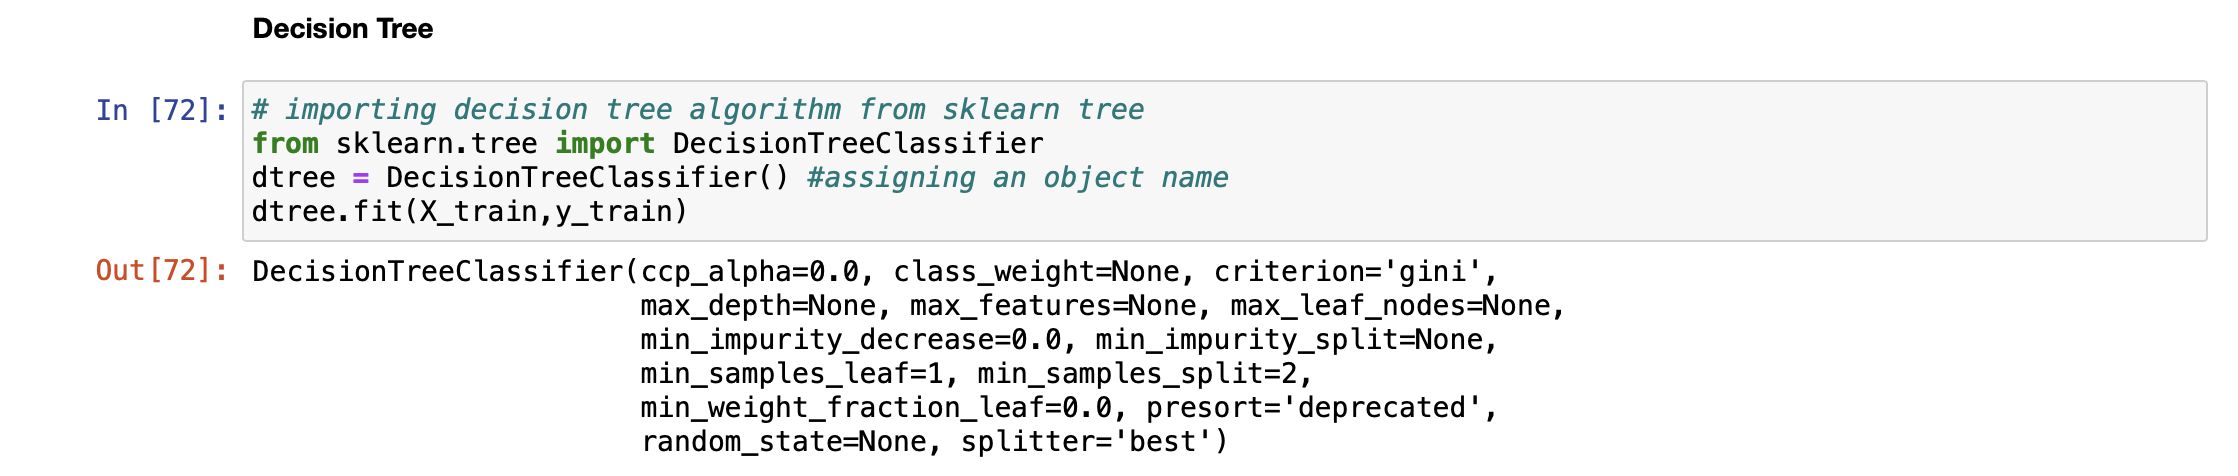
\includegraphics[scale=.4]{dt.png}}
\end{center}

The prediction is made as follows:

\begin{center}
\begin{figure}[h]
\centerline{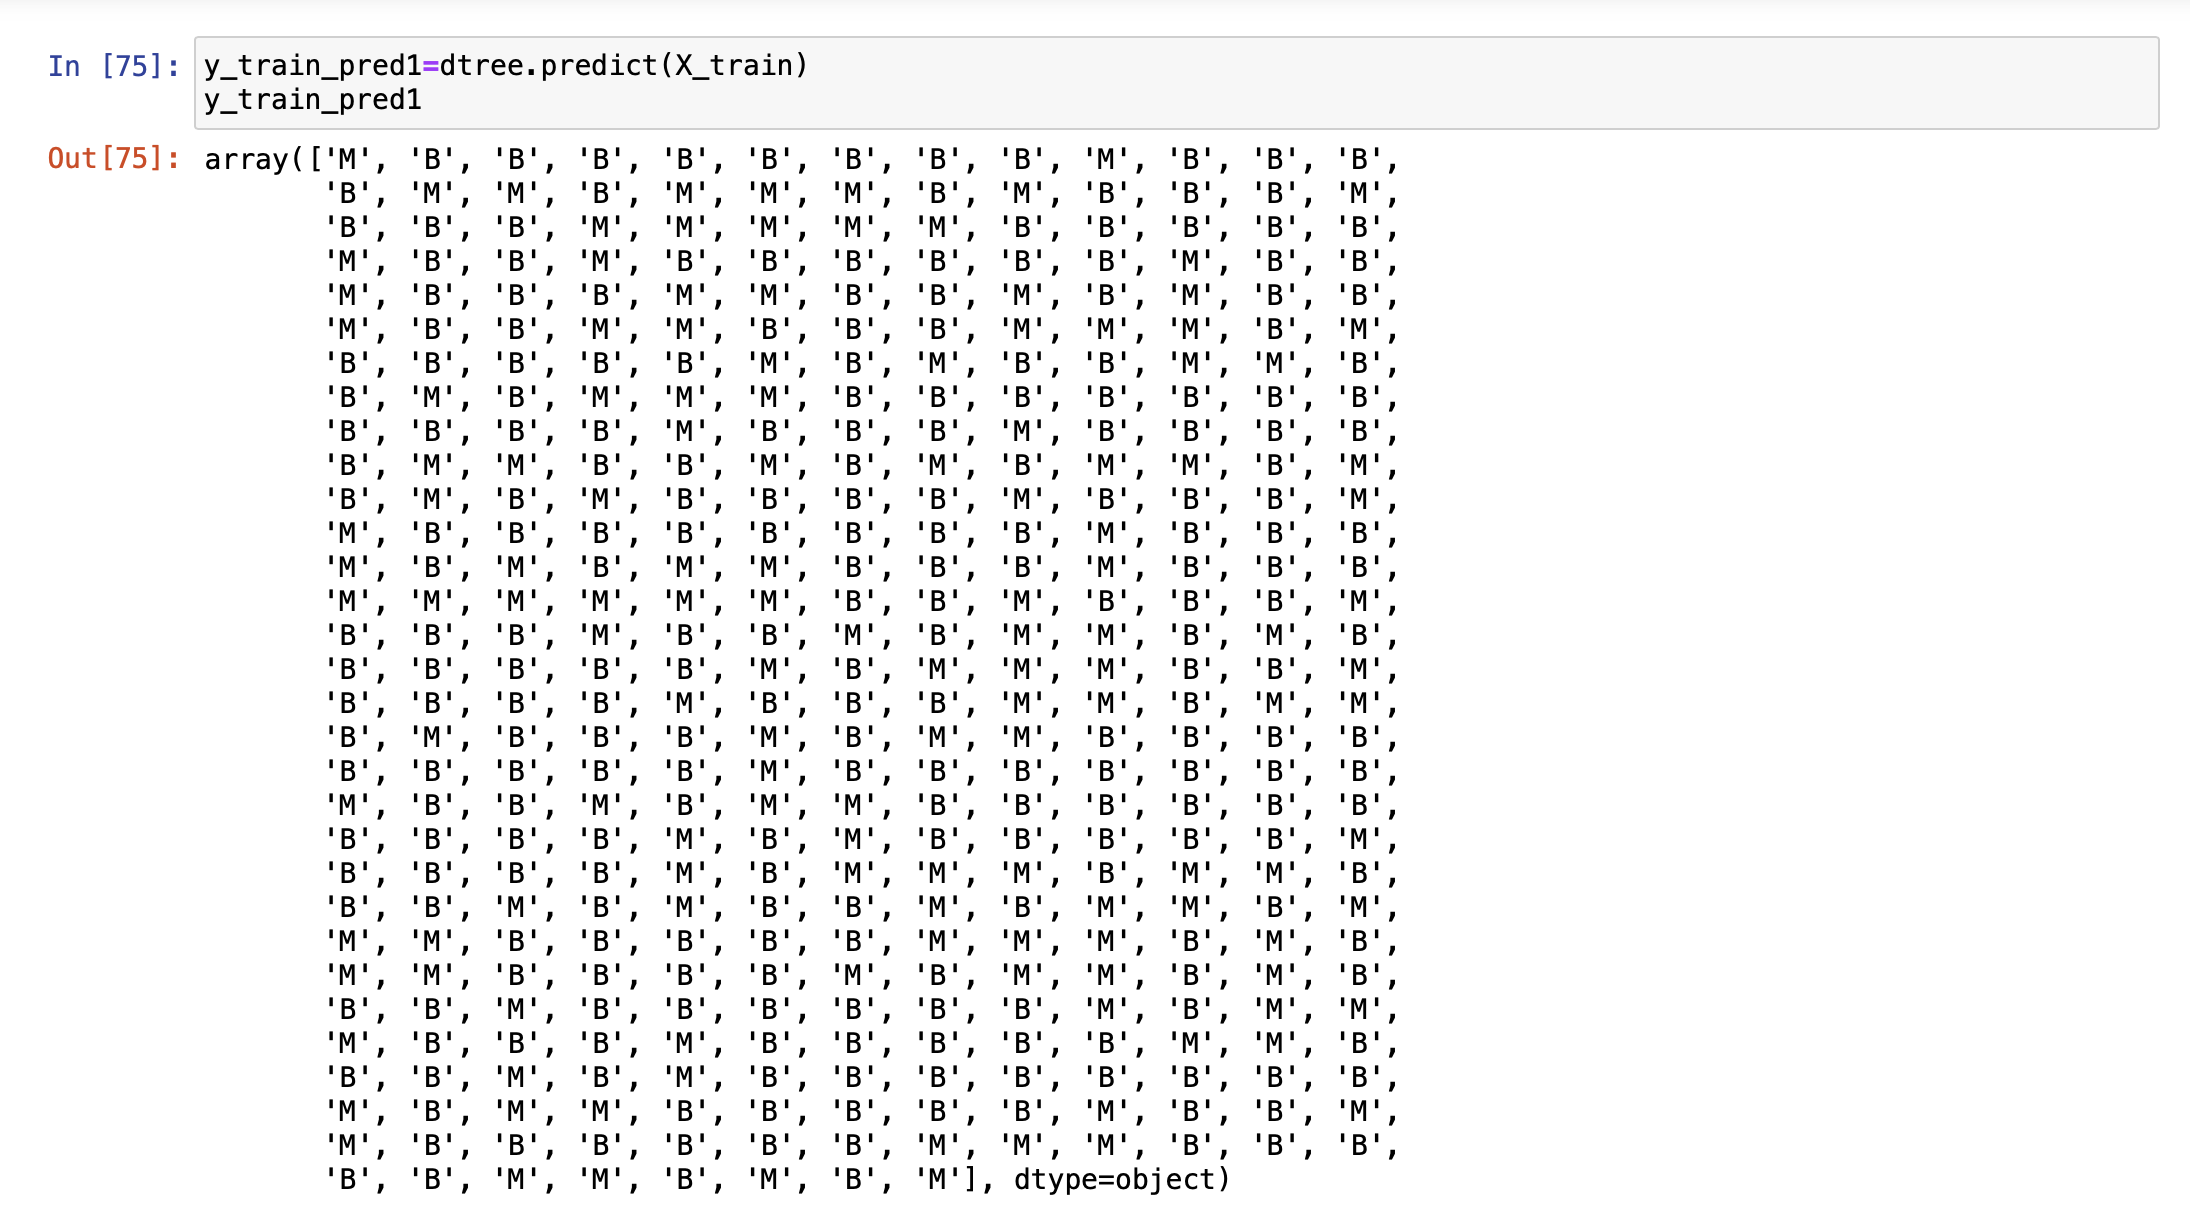
\includegraphics[scale=.4]{dtreepred.png}}
\caption{Decision Tree Prediction}
\end{figure}
\end{center}
\newpage 

\subsubsection{\textbf{RANDOM FORESTS }}
The random forest model is implemented using the RandomForestClassifier from the sklearn-ensemble model. The training and testing data is then fit to it as follows

\begin{center}
\centerline{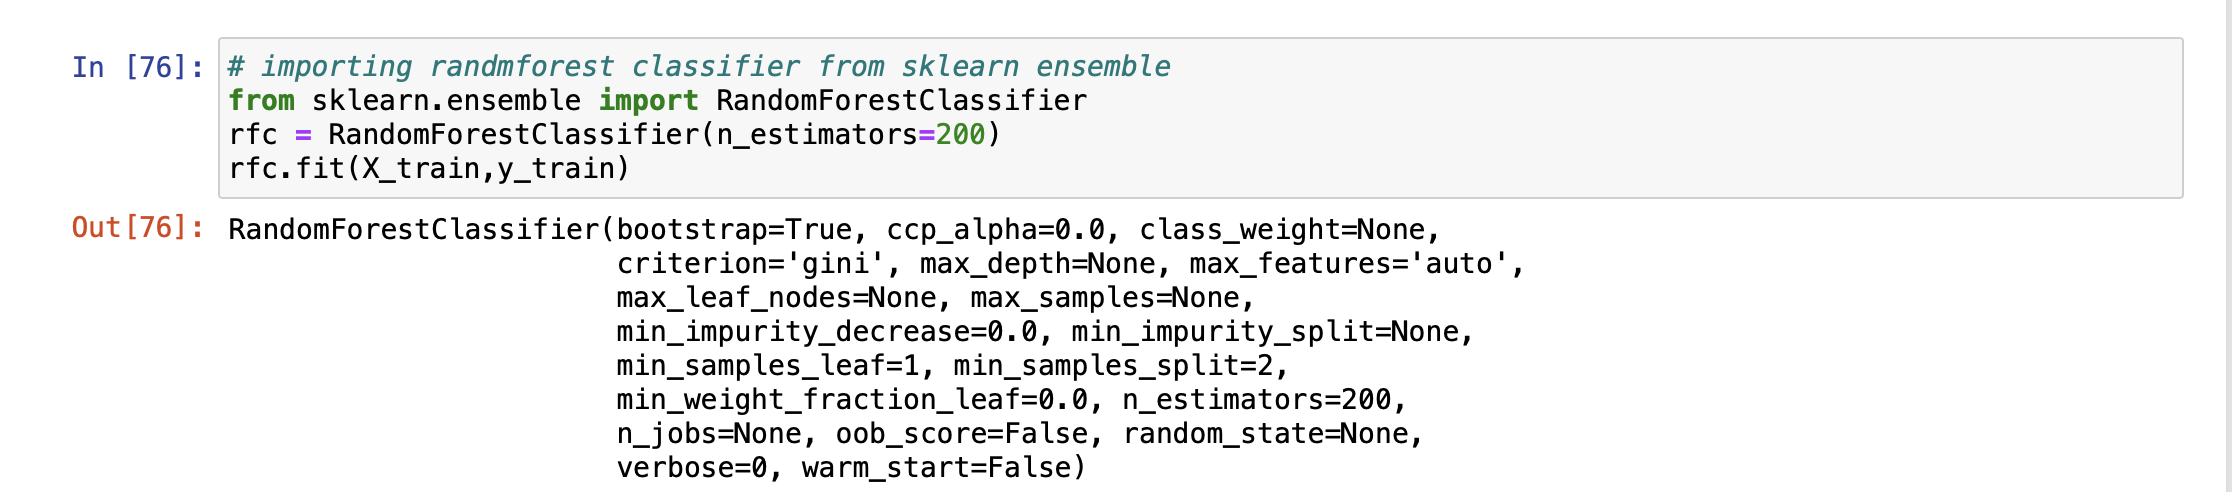
\includegraphics[scale=.4]{rf.png}}
\end{center}

The prediction is then made as follows 

\begin{center}
\begin{figure}[h]
\centerline{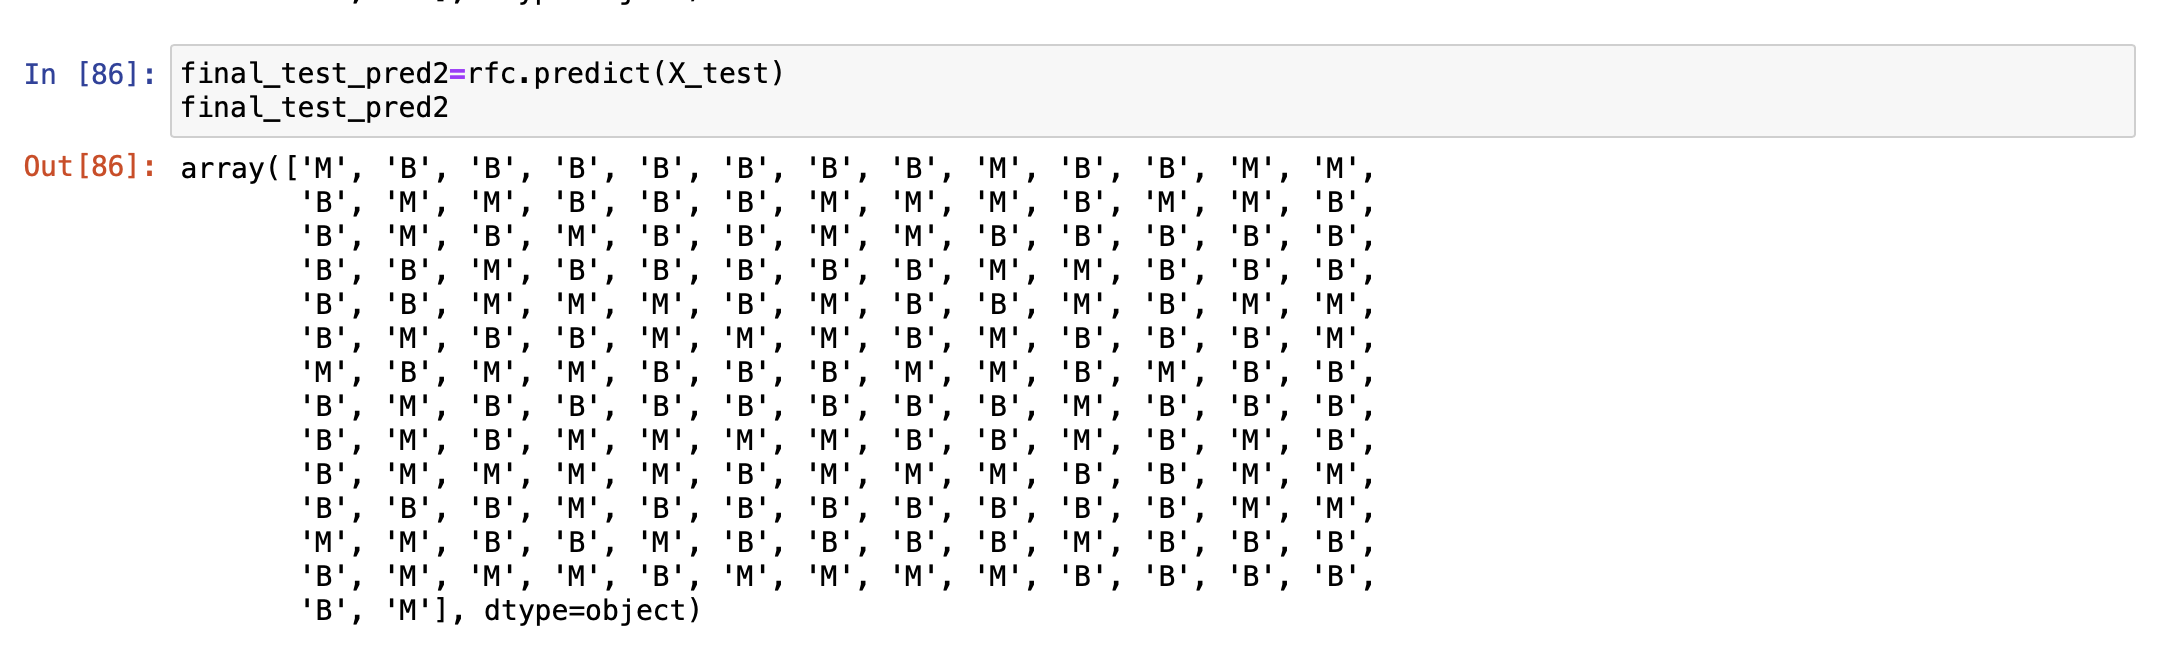
\includegraphics[scale=.4]{rfpred.png}}
\caption{Random Forest Prediction}
\end{figure}
\end{center}
\newpage 

\subsubsection{\textbf{SUPPORT VECTOR MACHINES }}
The support vector machines are implemented using the SVC class of the sklearn-svm model. The training and testing data is then fit to it as 

\begin{center}
\centerline{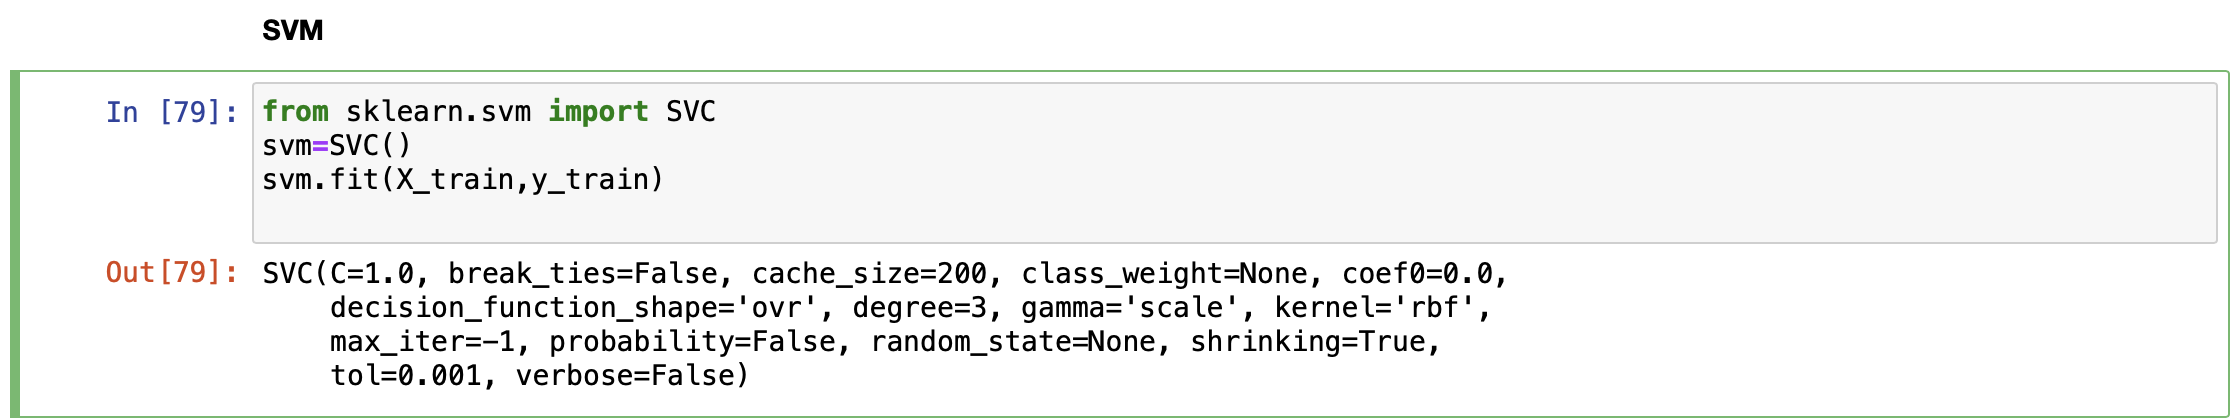
\includegraphics[scale=.4]{svm.png}}
\end{center}

The prediction is made as follows:

\begin{center}
\begin{figure}[h]
\centerline{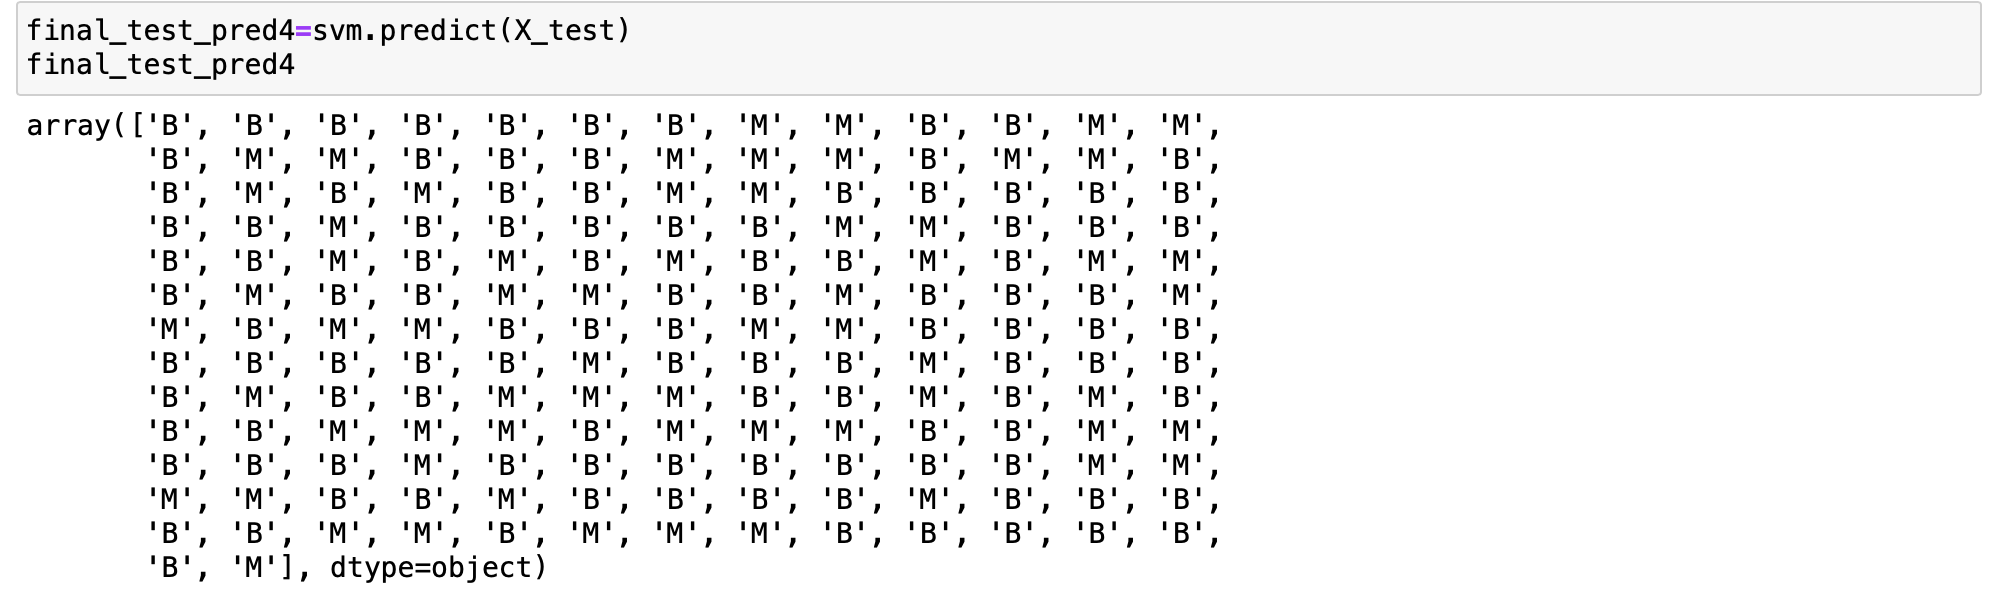
\includegraphics[scale=.4]{sv.png}}
\caption{Svm Prediction}
\end{figure}
\end{center}
\newpage
\section{\mainsize{\textbf{RESULT ANALYSIS}}}
Now we have concluded the training, testing and deployment of our models.
 After cross-validating the output of the models with the actual outputs from the dataset we have displayed the accuracy of each and every model 
\subsection{\msize{\textbf{PERFORMANCE SCORE OF EACH MODEL}}}
The performance score of each model are as follows : 

1. K Nearest Neighbours : This has got an accuracy score of 94\%
\begin{center}
\begin{figure}[h]
\centerline{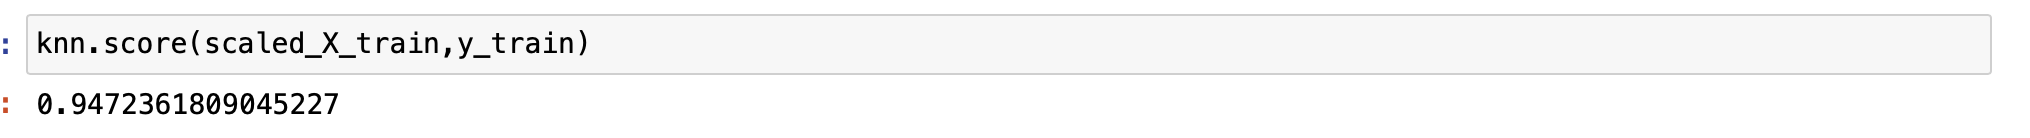
\includegraphics[scale=.45]{knnp.png}}
\caption{Knn Performance}
\end{figure}
\end{center}

2. Logistic Regression : This has got an accuracy score of 95\%
\begin{center}
\begin{figure}[h]
\centerline{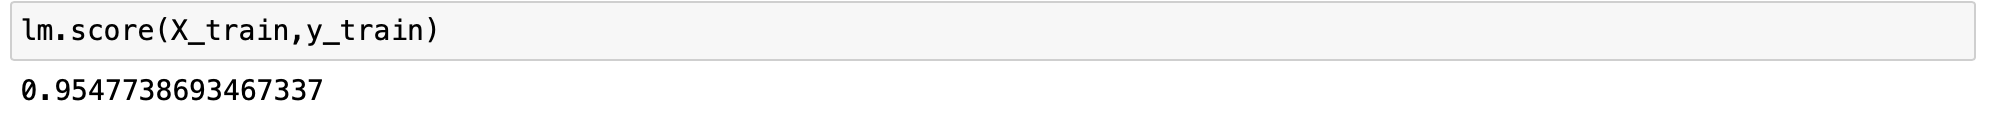
\includegraphics[scale=.45]{lrp.png}}
\caption{Logistic Performance}
\end{figure}
\end{center}


3. Decision Tree : This has got an accuracy score of 94\%
\begin{center}
\begin{figure}[h]
\centerline{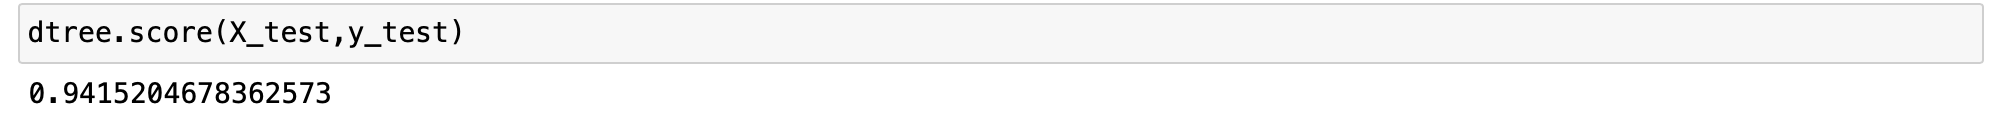
\includegraphics[scale=.45]{dtp.png}}
\caption{Decision Tree Performance}
\end{figure}
\end{center}

4. Random Forests :This has got an accuracy score of 95.9\%
\begin{center}
\begin{figure}[h]
\centerline{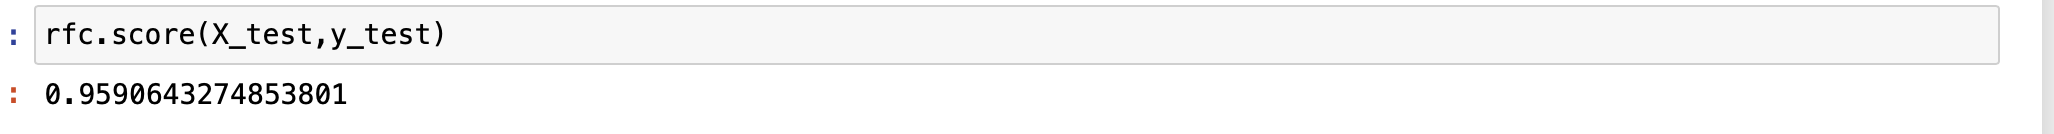
\includegraphics[scale=.45]{rfp.png}}
\caption{Random Forests Performance}
\end{figure}
\end{center}

5. Support Vector Machines : This has got an accuracy score of 90\%
\begin{center}
\begin{figure}[h]
\centerline{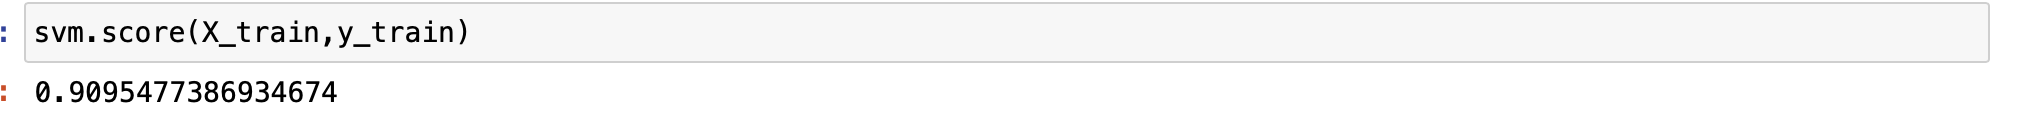
\includegraphics[scale=.45]{sp.png}}
\caption{Svm Performance}
\end{figure}
\end{center}


\subsection{\msize{\textbf{COMPARISION}}}
We have compared the models with the help of a bar chat. This par chart plots the accuracy scores of each model and displays it in an intuitive format 

\begin{center}
\begin{figure}[h]
\centerline{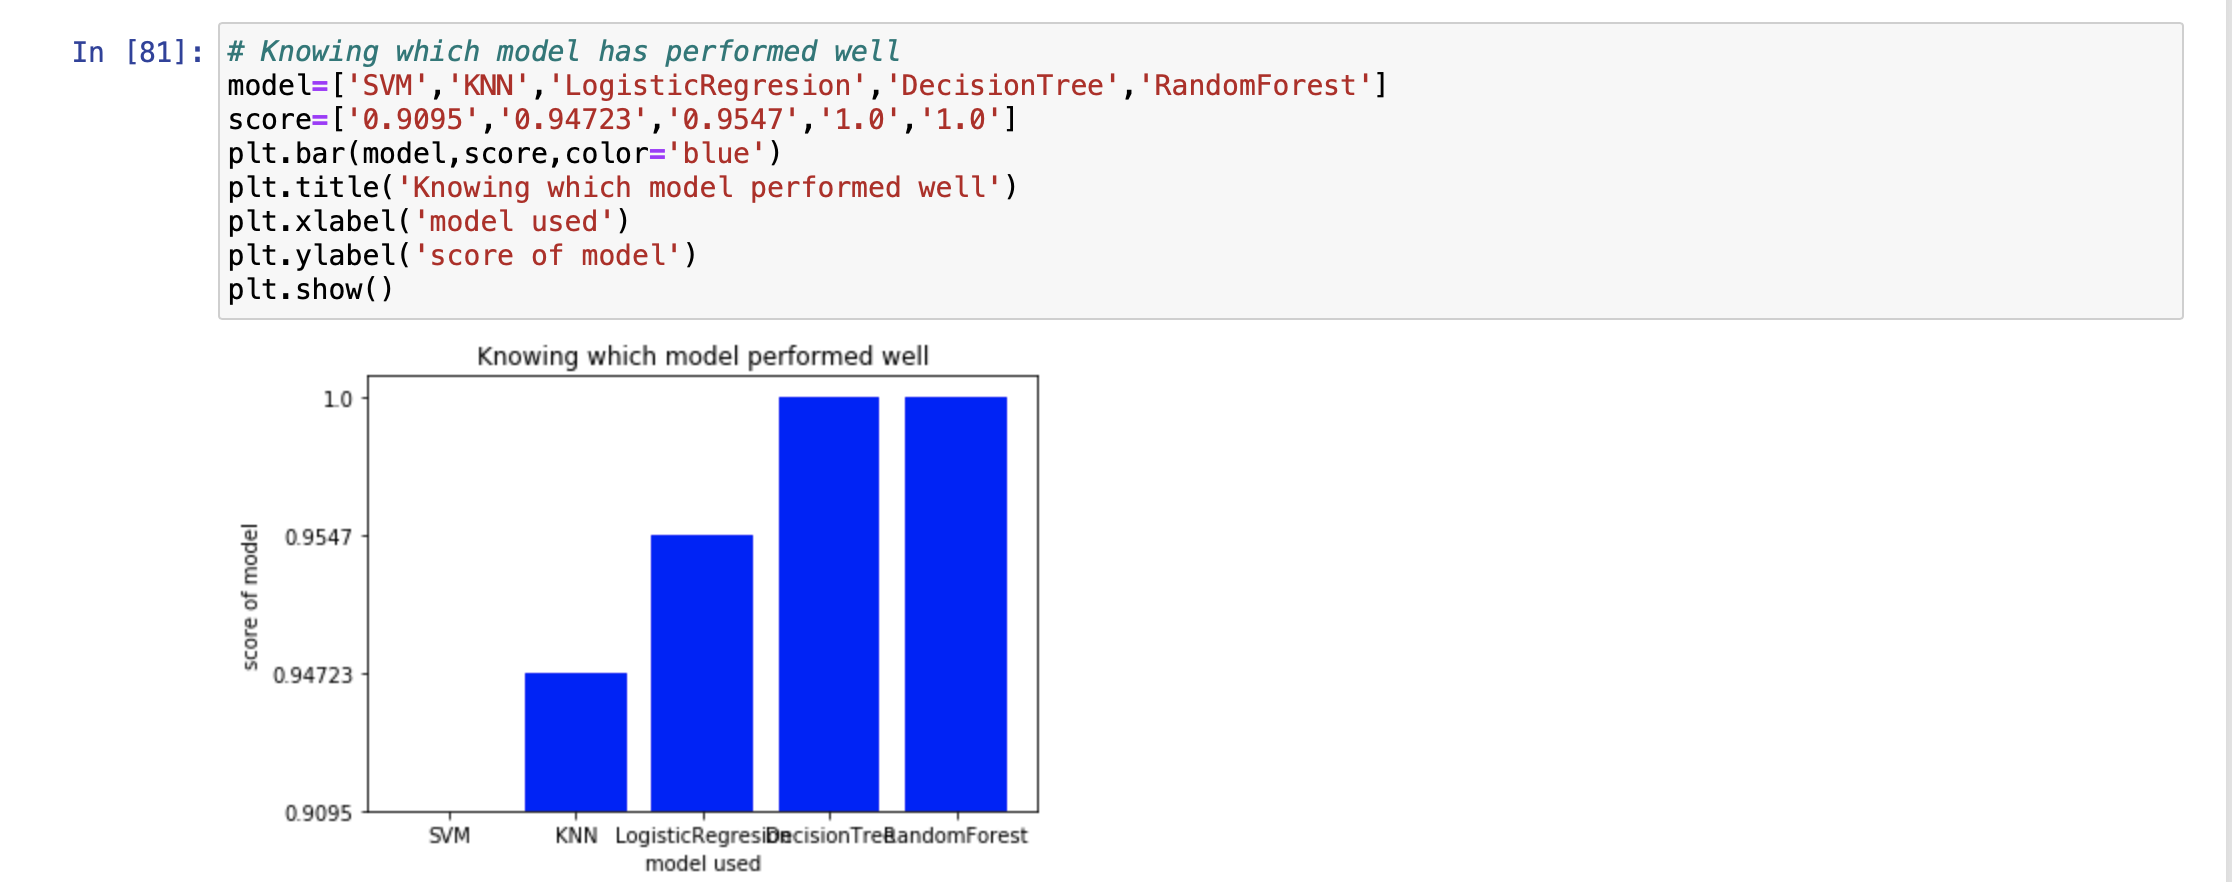
\includegraphics[scale=.4]{bar.png}}
\caption{Comparison}
\end{figure}
\end{center}

From this we can see that the Random Forest model has performed most accurately among all the deployed models
\newpage 
\section{\mainsize{\textbf{CONCLUSION}}}
The proposed model shows the overview of prediction of lung cancer at an early stage. After prediction of the tumour begins malignant or benign, we calculate accuracy score for each machine learning technique .
From the result we can say that our proposed model can distinguish between benign and malignant, and by comparing all the accuracy scores of machine learning techniques the best technique with highest accuracy score is selected i.e here Random Forest Classifier Algorithm has predicted well with a good accuracy for training data and testing data.

In future these models can be deployed remotely via a cloud network such as Amazon Web Services and can be used by multiple hospitals so detect whether a patient has malignant or benign cancer or not. This can help save numerous lives as the doctors can prevent the spread of the malignant tumour turning into lung cancer 
\newpage 
\section*{\mainsize{\textbf{REFERENCES}}}
\addcontentsline{toc}{section}{\protect\numberline{}\mainsize{\textbf{REFERENCES}}}
$[1]$ Lynch, Chip M., et al. "Prediction of lung cancer patient survival via supervised machine learning classification techniques." International
journal of medical informatics 108 (2017): 1-8.

\nd$[2]$   Fenwa, Olusayo D., Funmilola A. Ajala, and A. Adigun. "Classification of cancer of the lungs using SVM and ANN." Int. J.
 Comput. Technol. 15.1 (2016): 6418-6426.
 
\nd$[3]$ Öztürk, Şaban, and Bayram Akdemir. "Application of feature extraction and classification methods for histopathological image using GLCM, LBP, LBGLCM, GLRLM and SFTA."Procedia
computer science 132 (2018): 40-46.

\nd$[4]$ Jin, Xin-Yu, Yu-Chen Zhang, and Qi-Liang Jin. "Pulmonary nodule detection based on CT images using convolution neural network." 2016 9th International symposium on computational
intelligence and design (ISCID). Vol. 1. IEEE, 2016.

\nd$[5]$ Sumathipala, Yohan, et al. "Machine learning to predict lung nodule biopsy method using CT image features: A pilot study." Computerized Medical Imaging and Graphics 71 (2019): 1-8.

\nd$[6]$ Github repository : https://raw.githubusercontent.com/Mounika-Kajjam
                                            
\end{document}